\documentclass[swedish]{beamer}
\usepackage{pgfpages}
\usepackage{myslides}
\usepackage{fancyvrb}
\usepackage[lighttt]{lmodern}
\usepackage{menukeys}
\lstset{language=bash}

\makeatletter
\AtBeginDocument{% 
   \@ifpackageloaded{fancyvrb}{}{\let\@xpace@fancyvrb@catcodes\relax}% 

} 

\def\@xpace@fancyvrb@catcodes{% 
   \ifx\relax \FV@CommandChars 
   \else 
     \expandafter\@xpace@fancyvrb@catcodes@aux\FV@CommandChars 
   \fi 
} 

\def\@xpace@fancyvrb@catcodes@aux 
   \catcode`#1=0\relax\catcode`#2=1\relax\catcode`#3=2\relax{% 
     \@makeother#1\@makeother#2\@makeother#3% 
} 

\def\@xspace@eTeX@setup{% 
   \begingroup 
   \everyeof{}% 
   \endlinechar=-1\relax 
   \@xpace@fancyvrb@catcodes % extra line here. 
   \catcode`\ =10\relax 
   \makeatletter 
   \catcode`\\\z@ 
   \catcode`\{\@ne 
   \catcode`\}\tw@ 
   \expandafter\scantokens\expandafter{\expandafter\gdef 
     \expandafter\@xspace@exceptions@tlp 
     \expandafter{\@xspace@exceptions@tlp}}% 
   \endgroup 
} 
\makeatother

\newenvironment{dialogue}{%
\VerbatimEnvironment
\begin{Verbatim}[fontsize=\footnotesize,commandchars=\#\(\)]%
}
{%
\end{Verbatim}
}

\title{Versionshantering och git}
\author{Kai-Mikael Jää-Aro}
\date{}


\begin{document}
\setlength{\intextsep}{0mm}
%\setbeameroption{show notes on second screen=left}

\begin{frame}
\titlepage
\end{frame}

\begin{frame}
  \frametitle{Versionskontroll}
Mjukvaruutveckling är inte en linjär process från en tom fil till \(n\) rader korrekt fungerande kod.
\begin{itemize}
\item Fel införs under arbetets gång.
\item Vi provar alternativa lösningar.
\item Flera parallella versioner krävs.
\end{itemize}

Därför måste vi:
\begin{itemize}
\item kunna återgå till en fungerande version av mjukvaran,
\item arbeta med en av flera möjliga versioner.
\end{itemize}

En lösning på detta problem är \emph{versionskontroll}.
\end{frame}

\begin{frame}
  \begin{itemize}
  \item Ett arkiv
  \item\emph{Incheckning} av kod (\emph{revisioner}) i arkivet.
\note[item]{Incheckningen ska också ha kommentar om vad som ändrats sen sist.}
  \item  Trädstruktur för parallella versioner 
  \item Hämta ut tidigare incheckningar
  \end{itemize}
\end{frame}

\begin{frame}
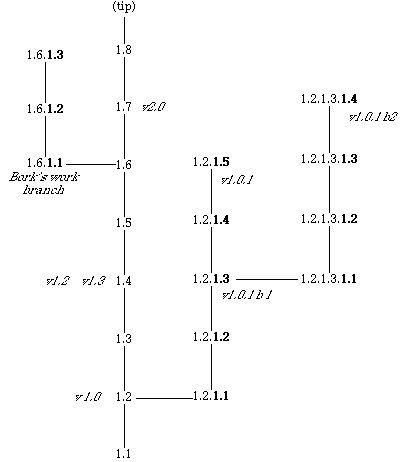
\includegraphics[height=0.8\textheight]{revision-tree}
\end{frame}

\begin{frame}
``tip''/``trunk''/``master'' är huvudspåret.

Varje revision har en identitet, kan markeras med en \emph{tag} som 
motsvarar släppt version eller annan milsten.

Ändringar i parallella versioner kan föras tillbaka till master.
\end{frame}

\begin{frame}
\frametitle{Parallell utveckling}

Flera utvecklare i samma projekt.
\begin{enumerate}
\item Checka ut aktuell version av koden.
\item Koda, testa.
\item Checka in \emph{stabil} kod.
\item Hantera ev konflikter.
\item Repetera tills projektet klart.
\end{enumerate}
\end{frame}

\begin{frame}[fragile]
  \frametitle{Konflikthantering}
Antag att två kodare checkar in varsin version av metoden \lstinline+func1+:
\begin{tabular}{ll}
Kodare 1&Kodare 2\\
\begin{minipage}[t]{0.45\linewidth}
\begin{lstlisting}[basicstyle=\tiny]
public int func1(int par) {
  int var1 = 0;  // Ursprunglig rad
  var1 = par;   // Ny rad
  return(var1);
}
\end{lstlisting}
\end{minipage}
&
\begin{minipage}[t]{0.45\linewidth}
\begin{lstlisting}[basicstyle=\tiny]
public int func1(int par) {
  return(par);
}
\end{lstlisting}
\end{minipage}
\end{tabular}
\end{frame}

\begin{frame}[fragile]
Raden \lstinline+var1 = par;+ läggs till.
\lstinline+int var1 = 0;+ tas
bort.  

\lstinline+return+-satsen skiljer sig mellan de två incheckningarna, en \emph{konflikt}.  Denna måste lösas manuellt.

\end{frame}

\begin{frame}[fragile]
Versionshanteringssystemet förstår bara koden som en sträng text.
Överlappande ändringar i samma kod flaggas, men om någon skulle ändra
funktionshuvudet till \lstinline+public void func1(int par1, int
par2)+ invalideras alla anrop till \lstinline+func1+, men
versionshanteringssystemet ser inte detta.

Därför bör alla incheckningar följas av ett \emph{bygge}.
\end{frame}

\begin{frame}
\frametitle{Git}
Det finns ett stort antal versionshanteringssystem, här kommer vi att gå igenom git.

  git är ett \emph{distribuerat} versionskontrollsystem.  \Mao lagrar \emph{alla} utvecklare en (komprimerad) kopia av hela databasen, men normalt utser man ett specifikt arkiv till att vara ``origin'', till vilket alla kopierar sitt material och som alla hämtar ifrån.

Dock är man inte beroende av det centrala arkivet utan kan arbeta offline med sin kopia tills man får kontakt med arkivet igen.

\end{frame}

\begin{frame}
  \frametitle{Att använda git}
Grunden för git är ett kommndoradsgränssnitt, men det finns flera olika grafiska gränssnitt.

GitHub (\url{https://github.com/}) gör tillgängligt både ett webbgränssnitt till git och gratis server-utrymme för open source-projekt.

\end{frame}


\begin{frame}
\frametitle{Att skapa ett arkiv}
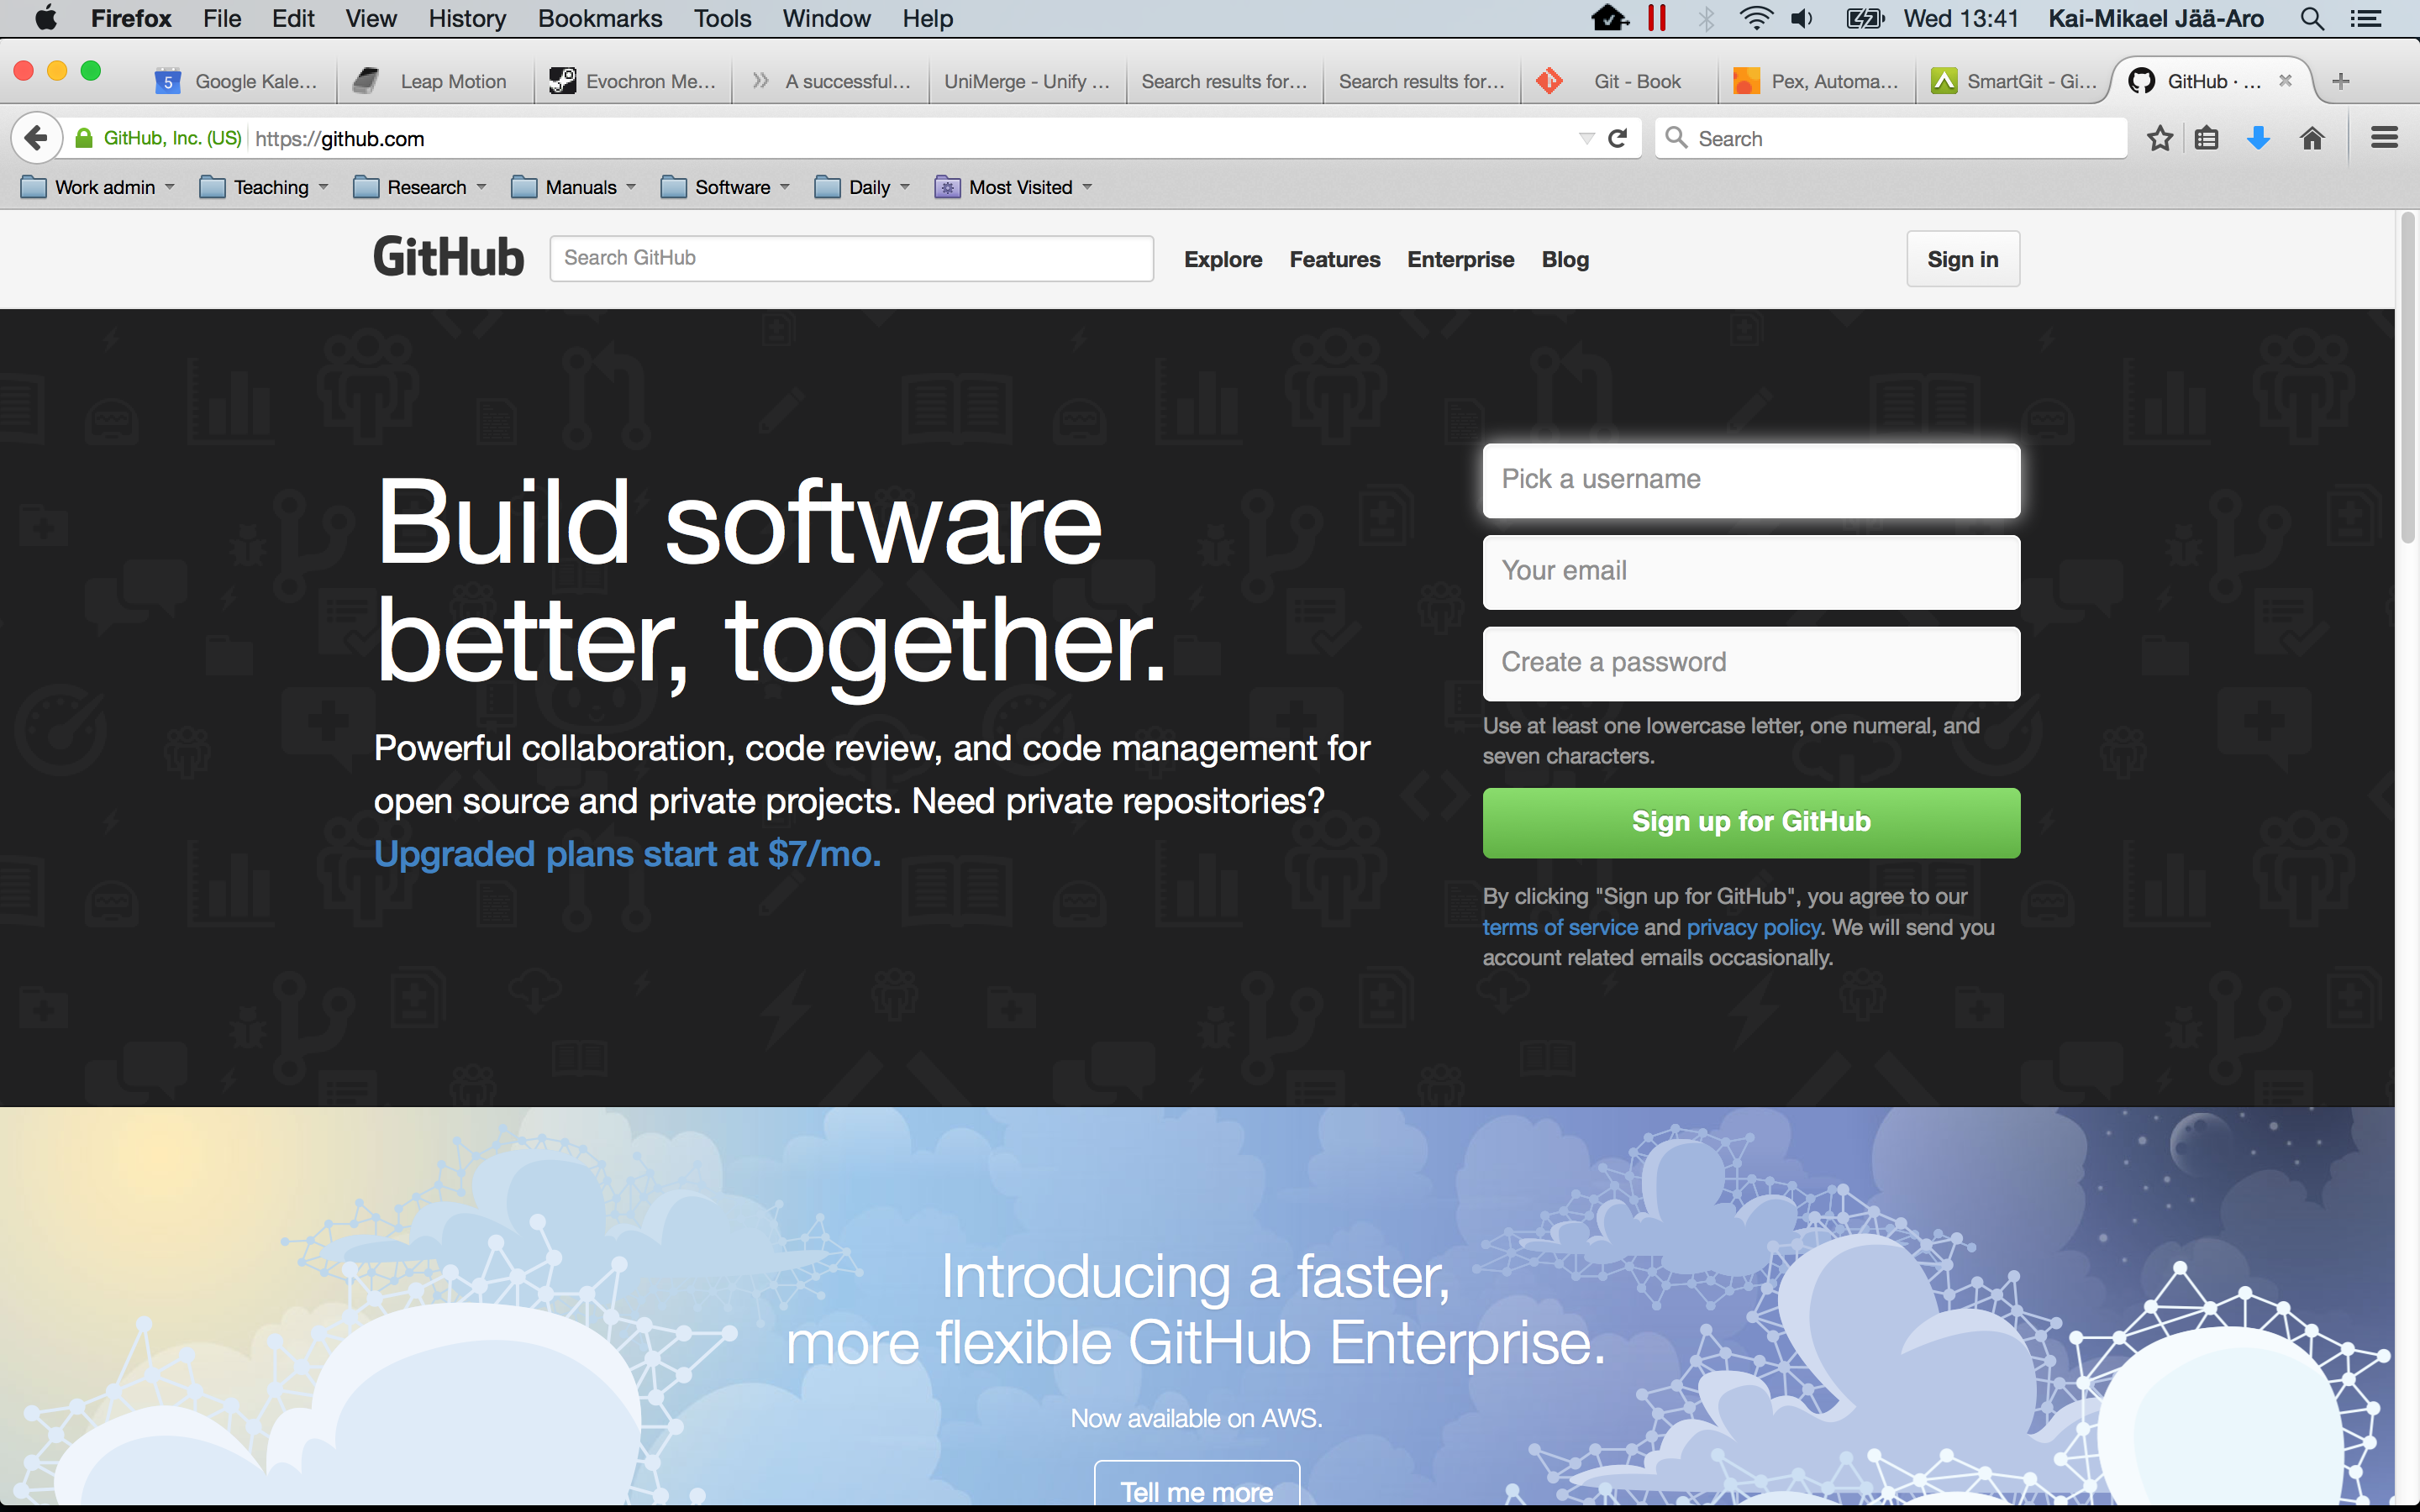
\includegraphics{GitHubSignUp}
\end{frame}

\begin{frame}[fragile]
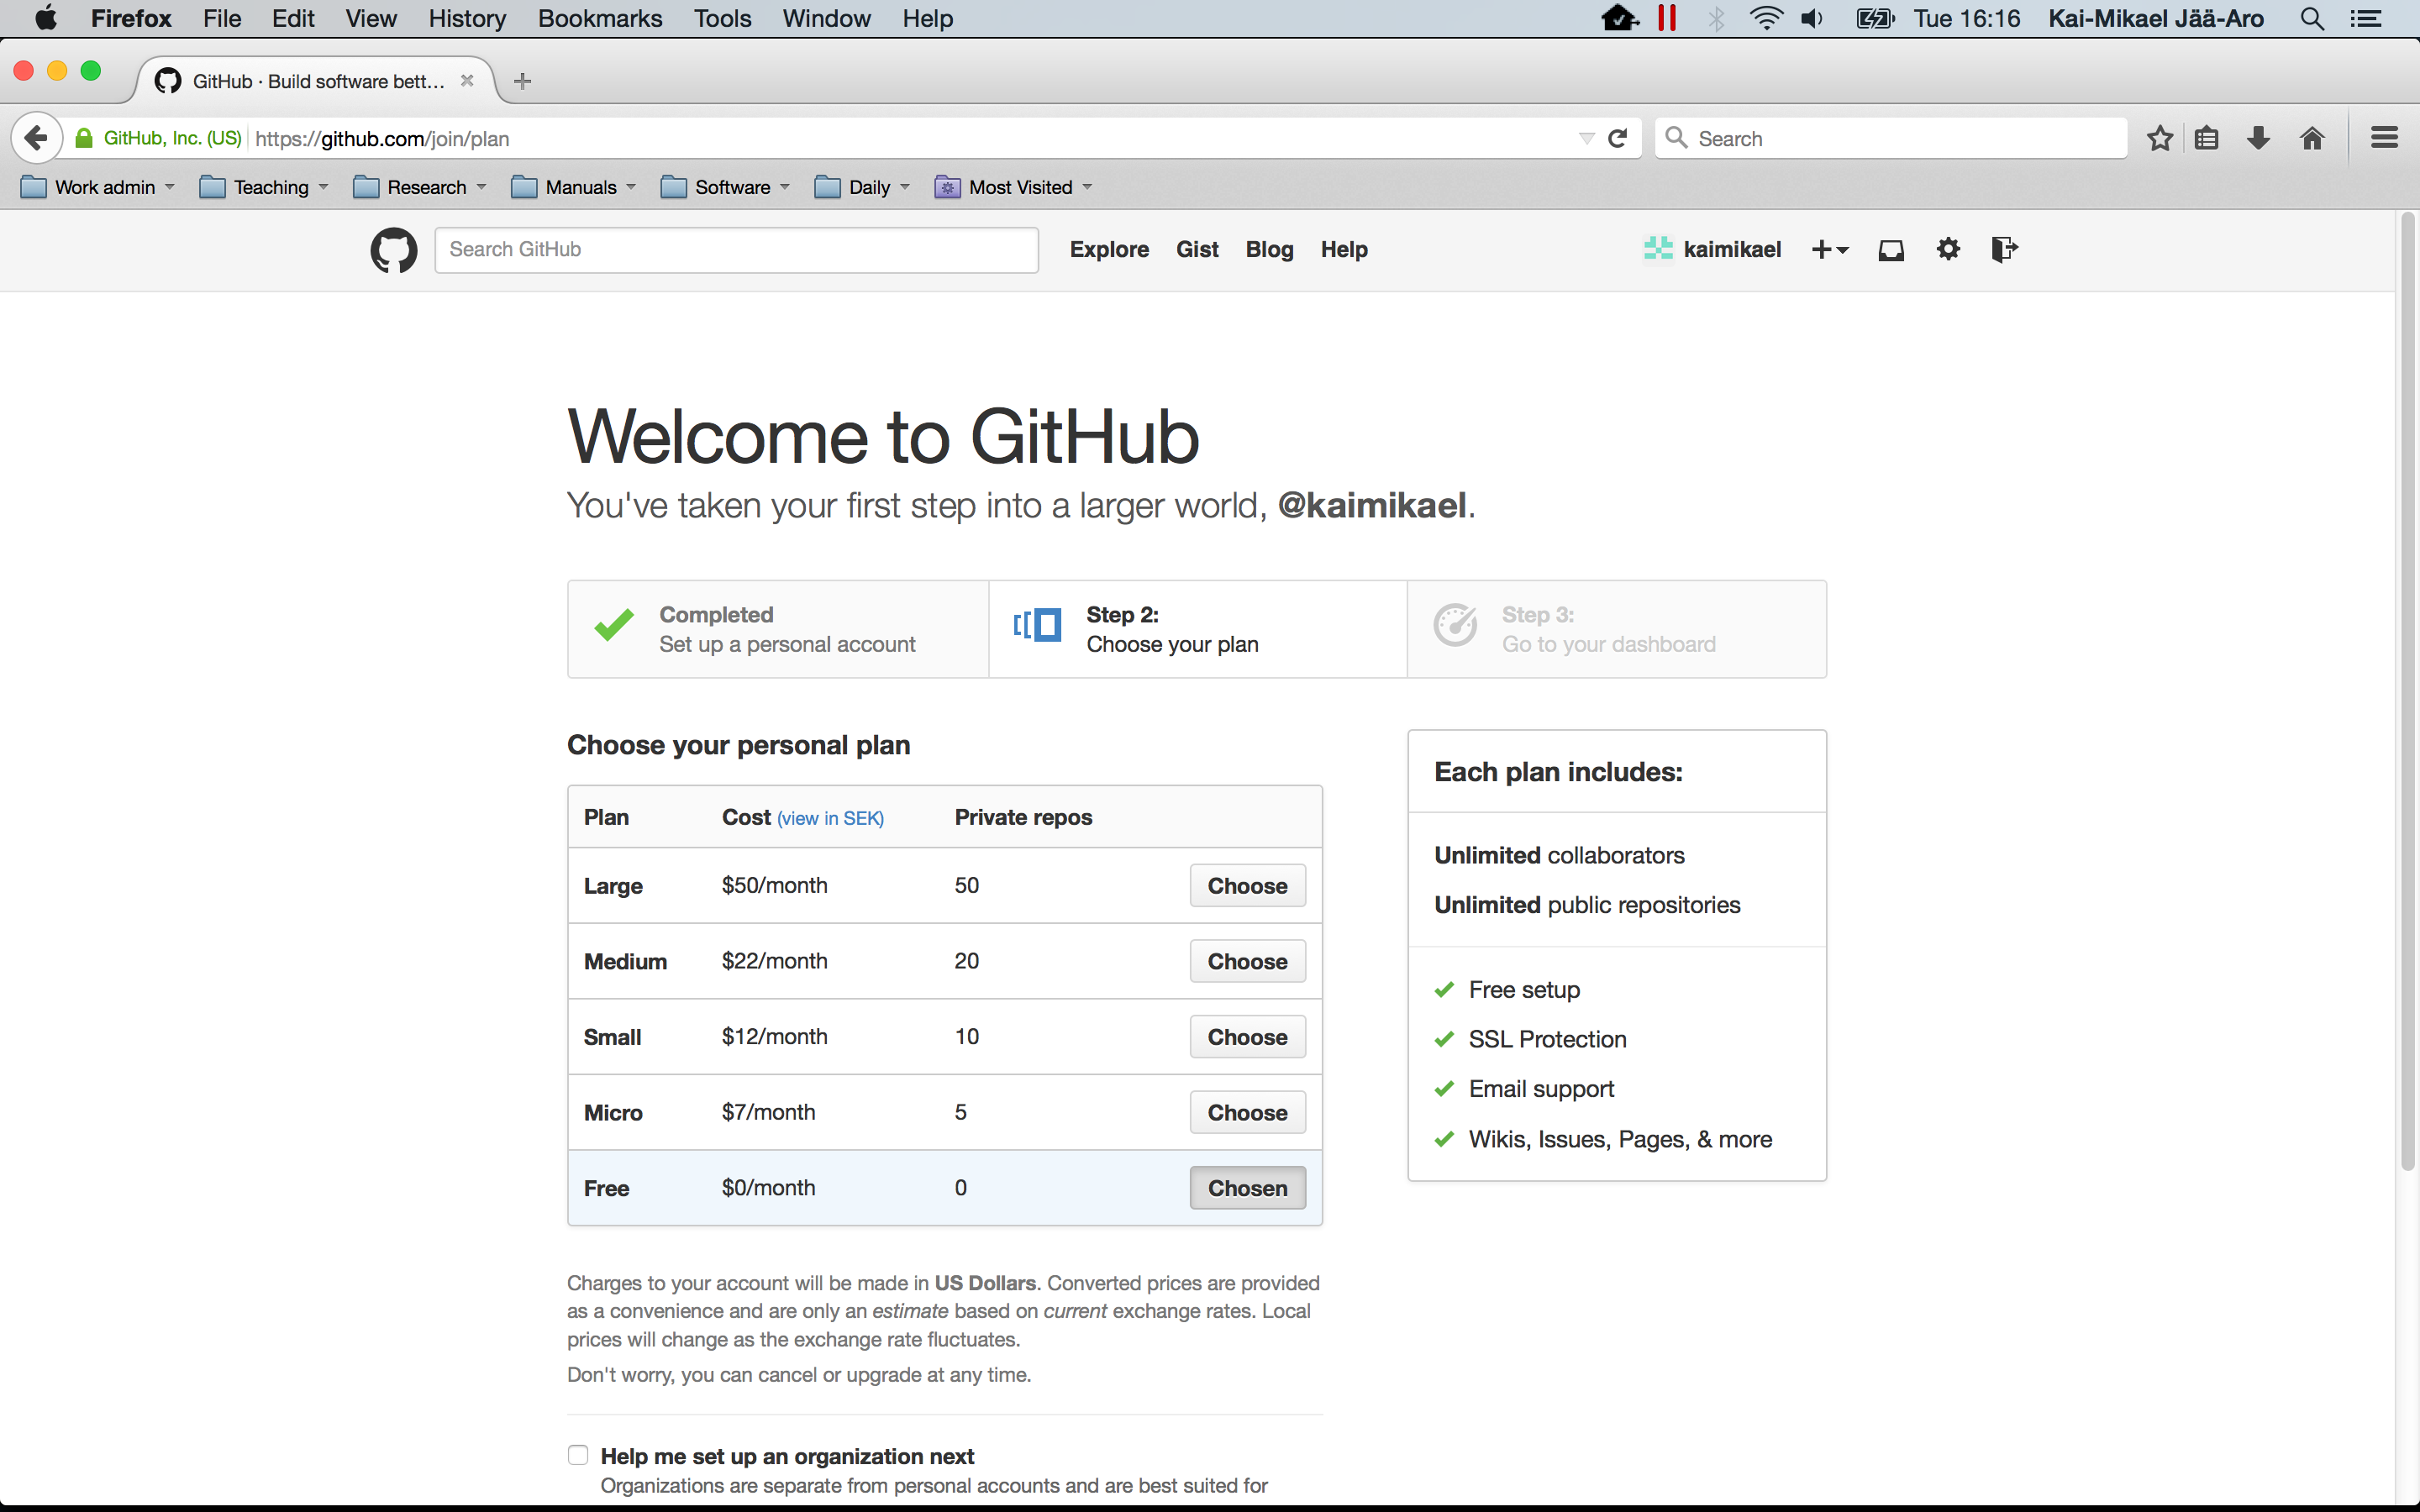
\includegraphics{ChoosePlan}
\end{frame}


\begin{frame}[fragile]
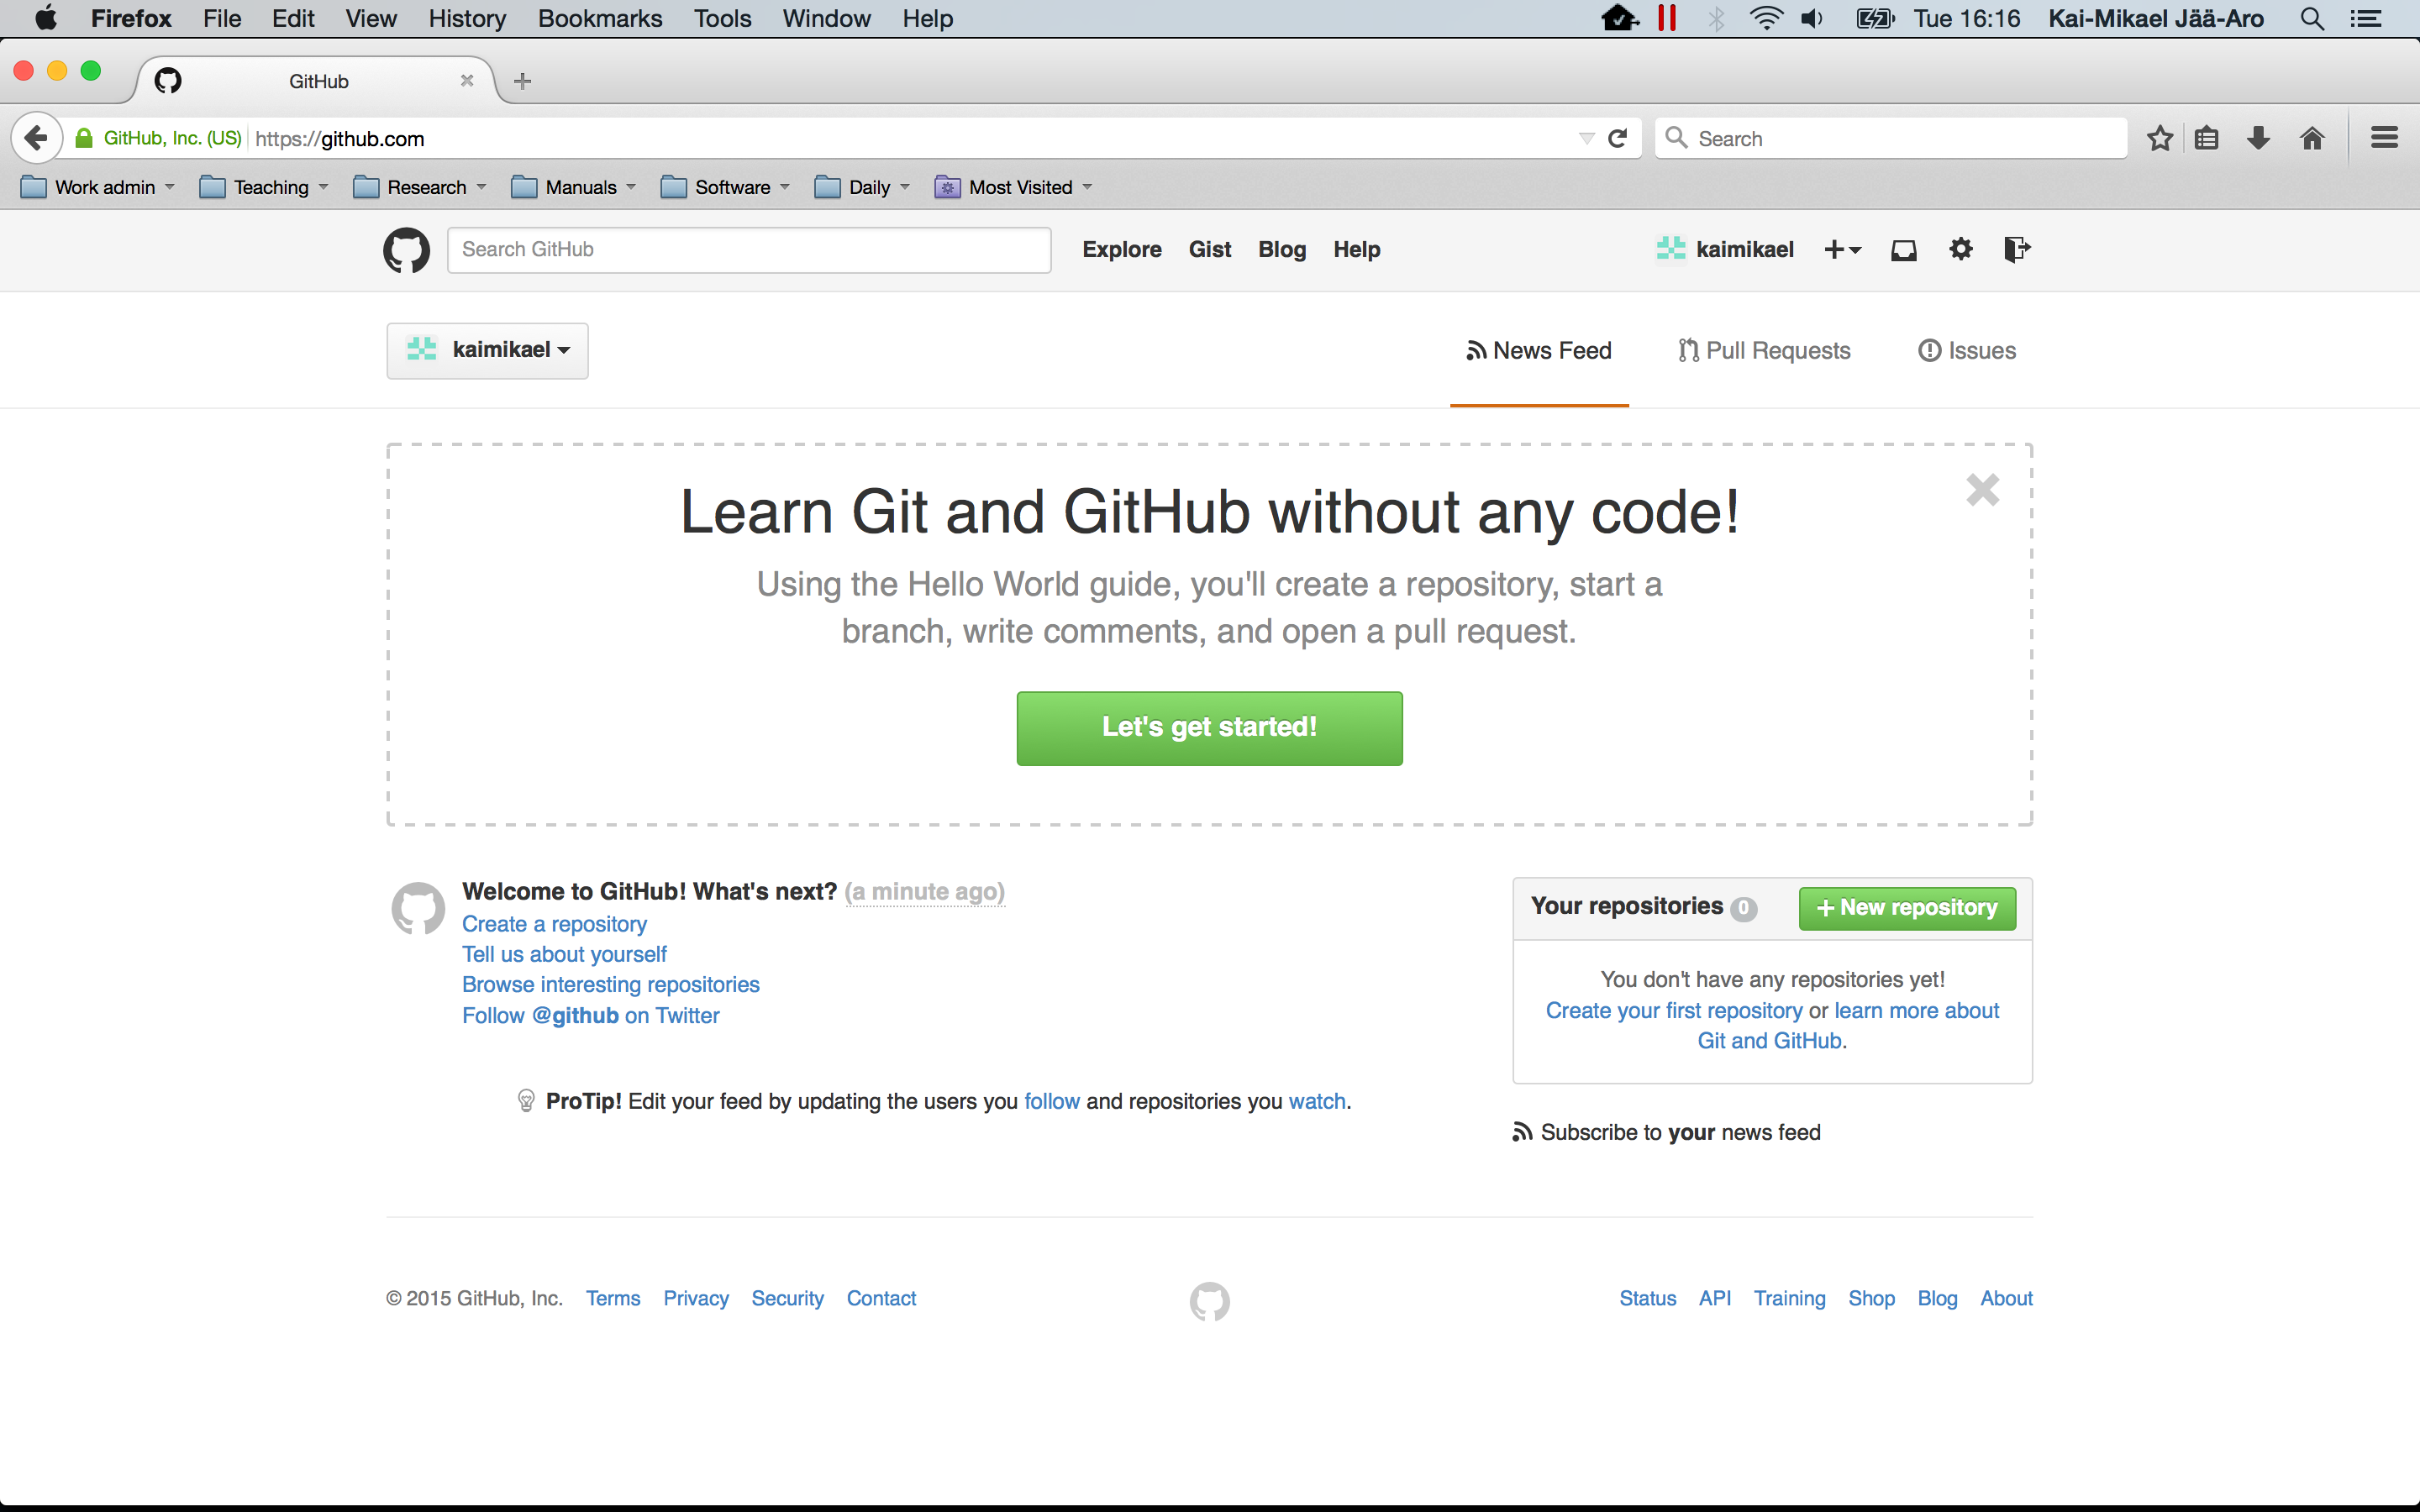
\includegraphics{CreateRepository}  
\end{frame}

\begin{frame}[fragile]
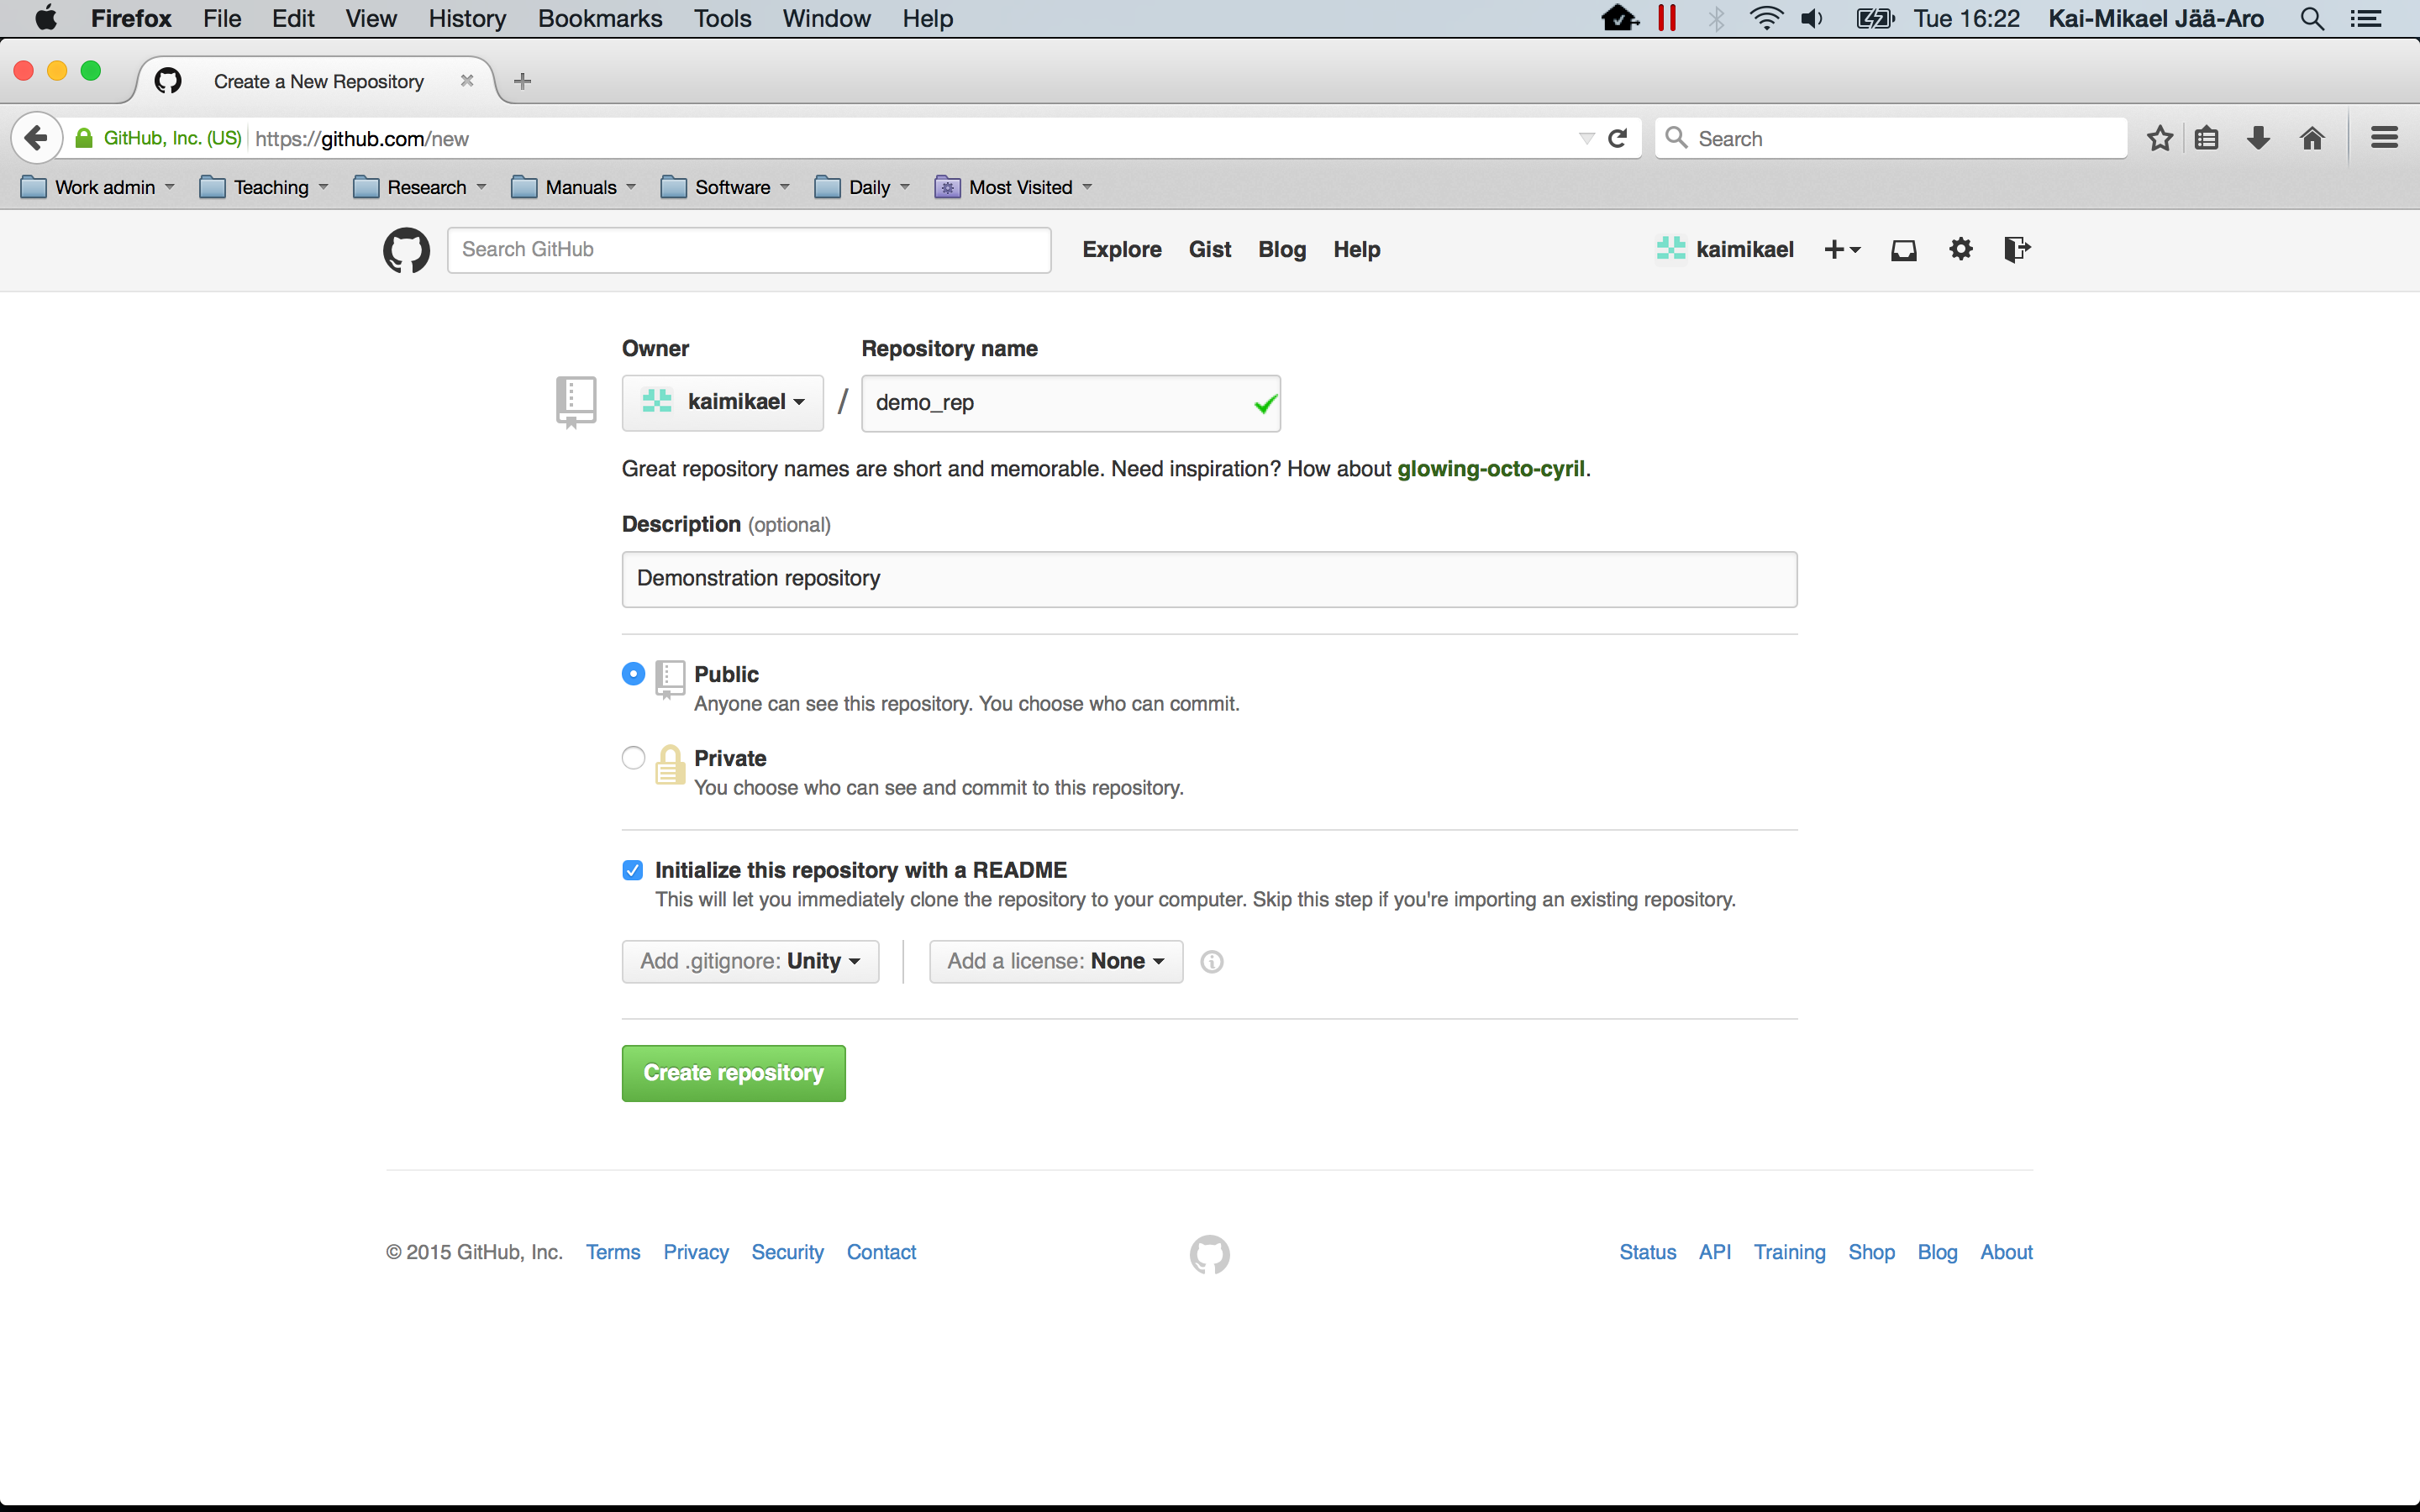
\includegraphics{NameRepository}
\end{frame}

\begin{frame}[fragile]
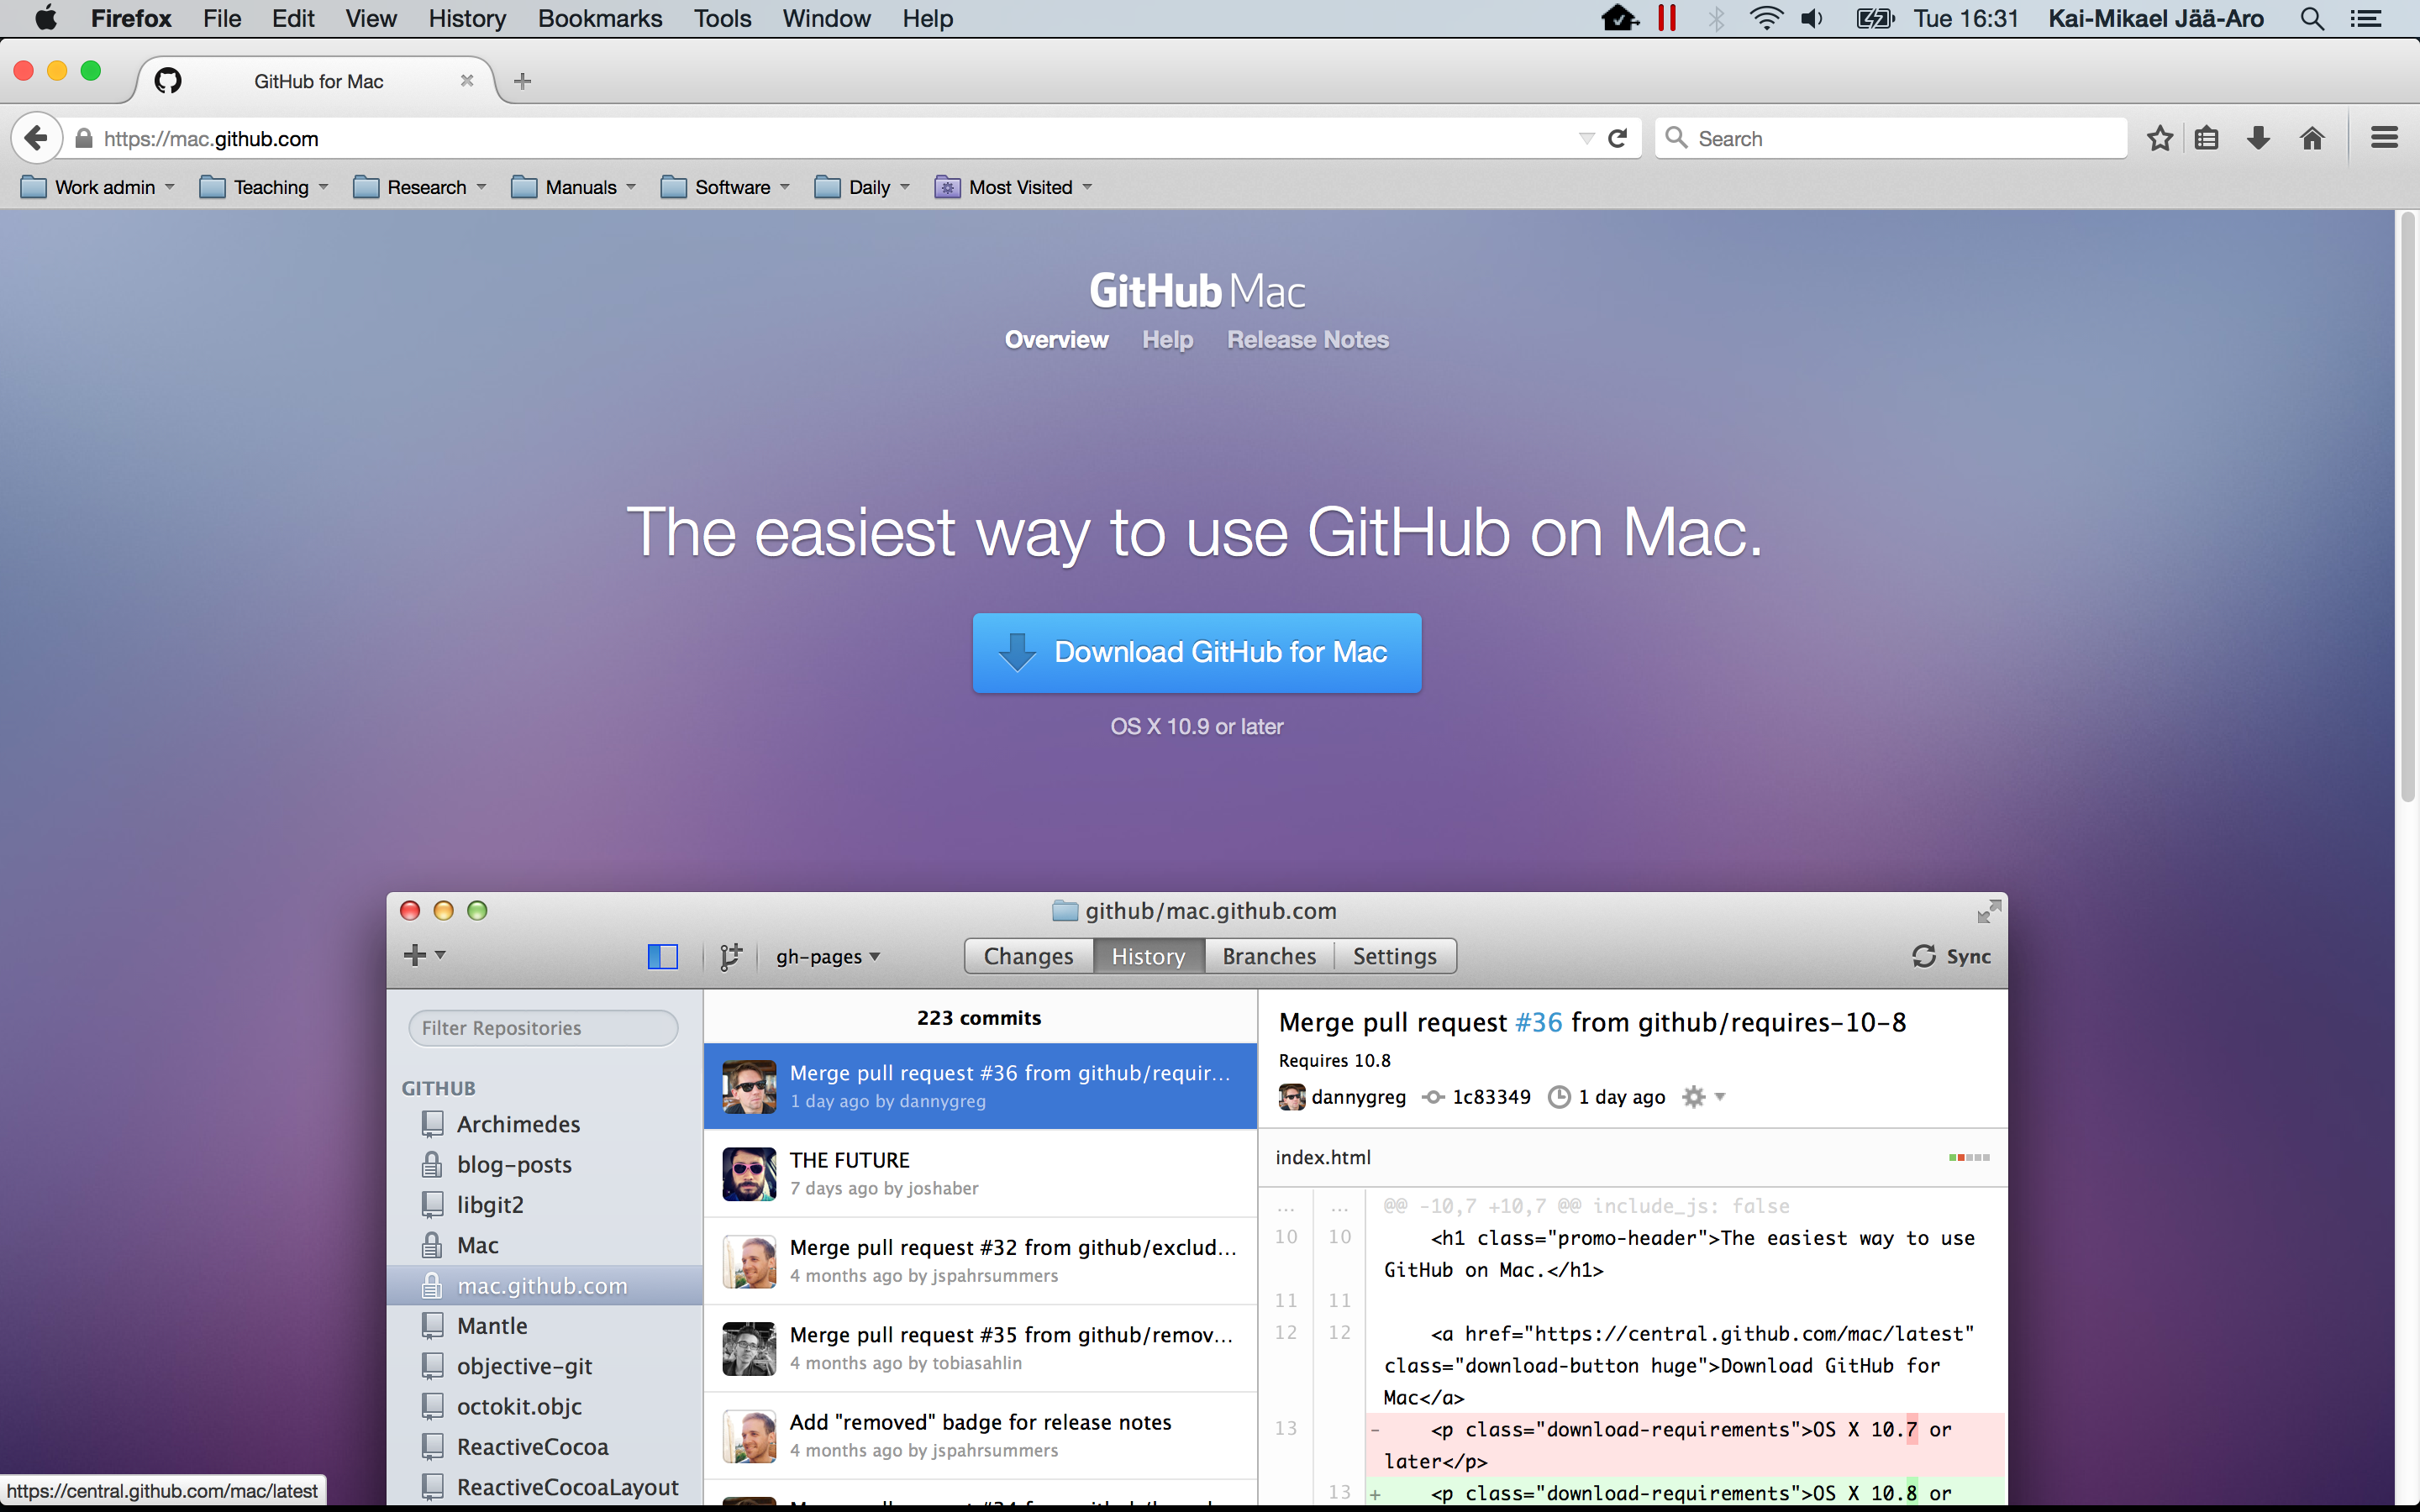
\includegraphics{GitHubDownload}

\end{frame}

\begin{frame}[fragile]
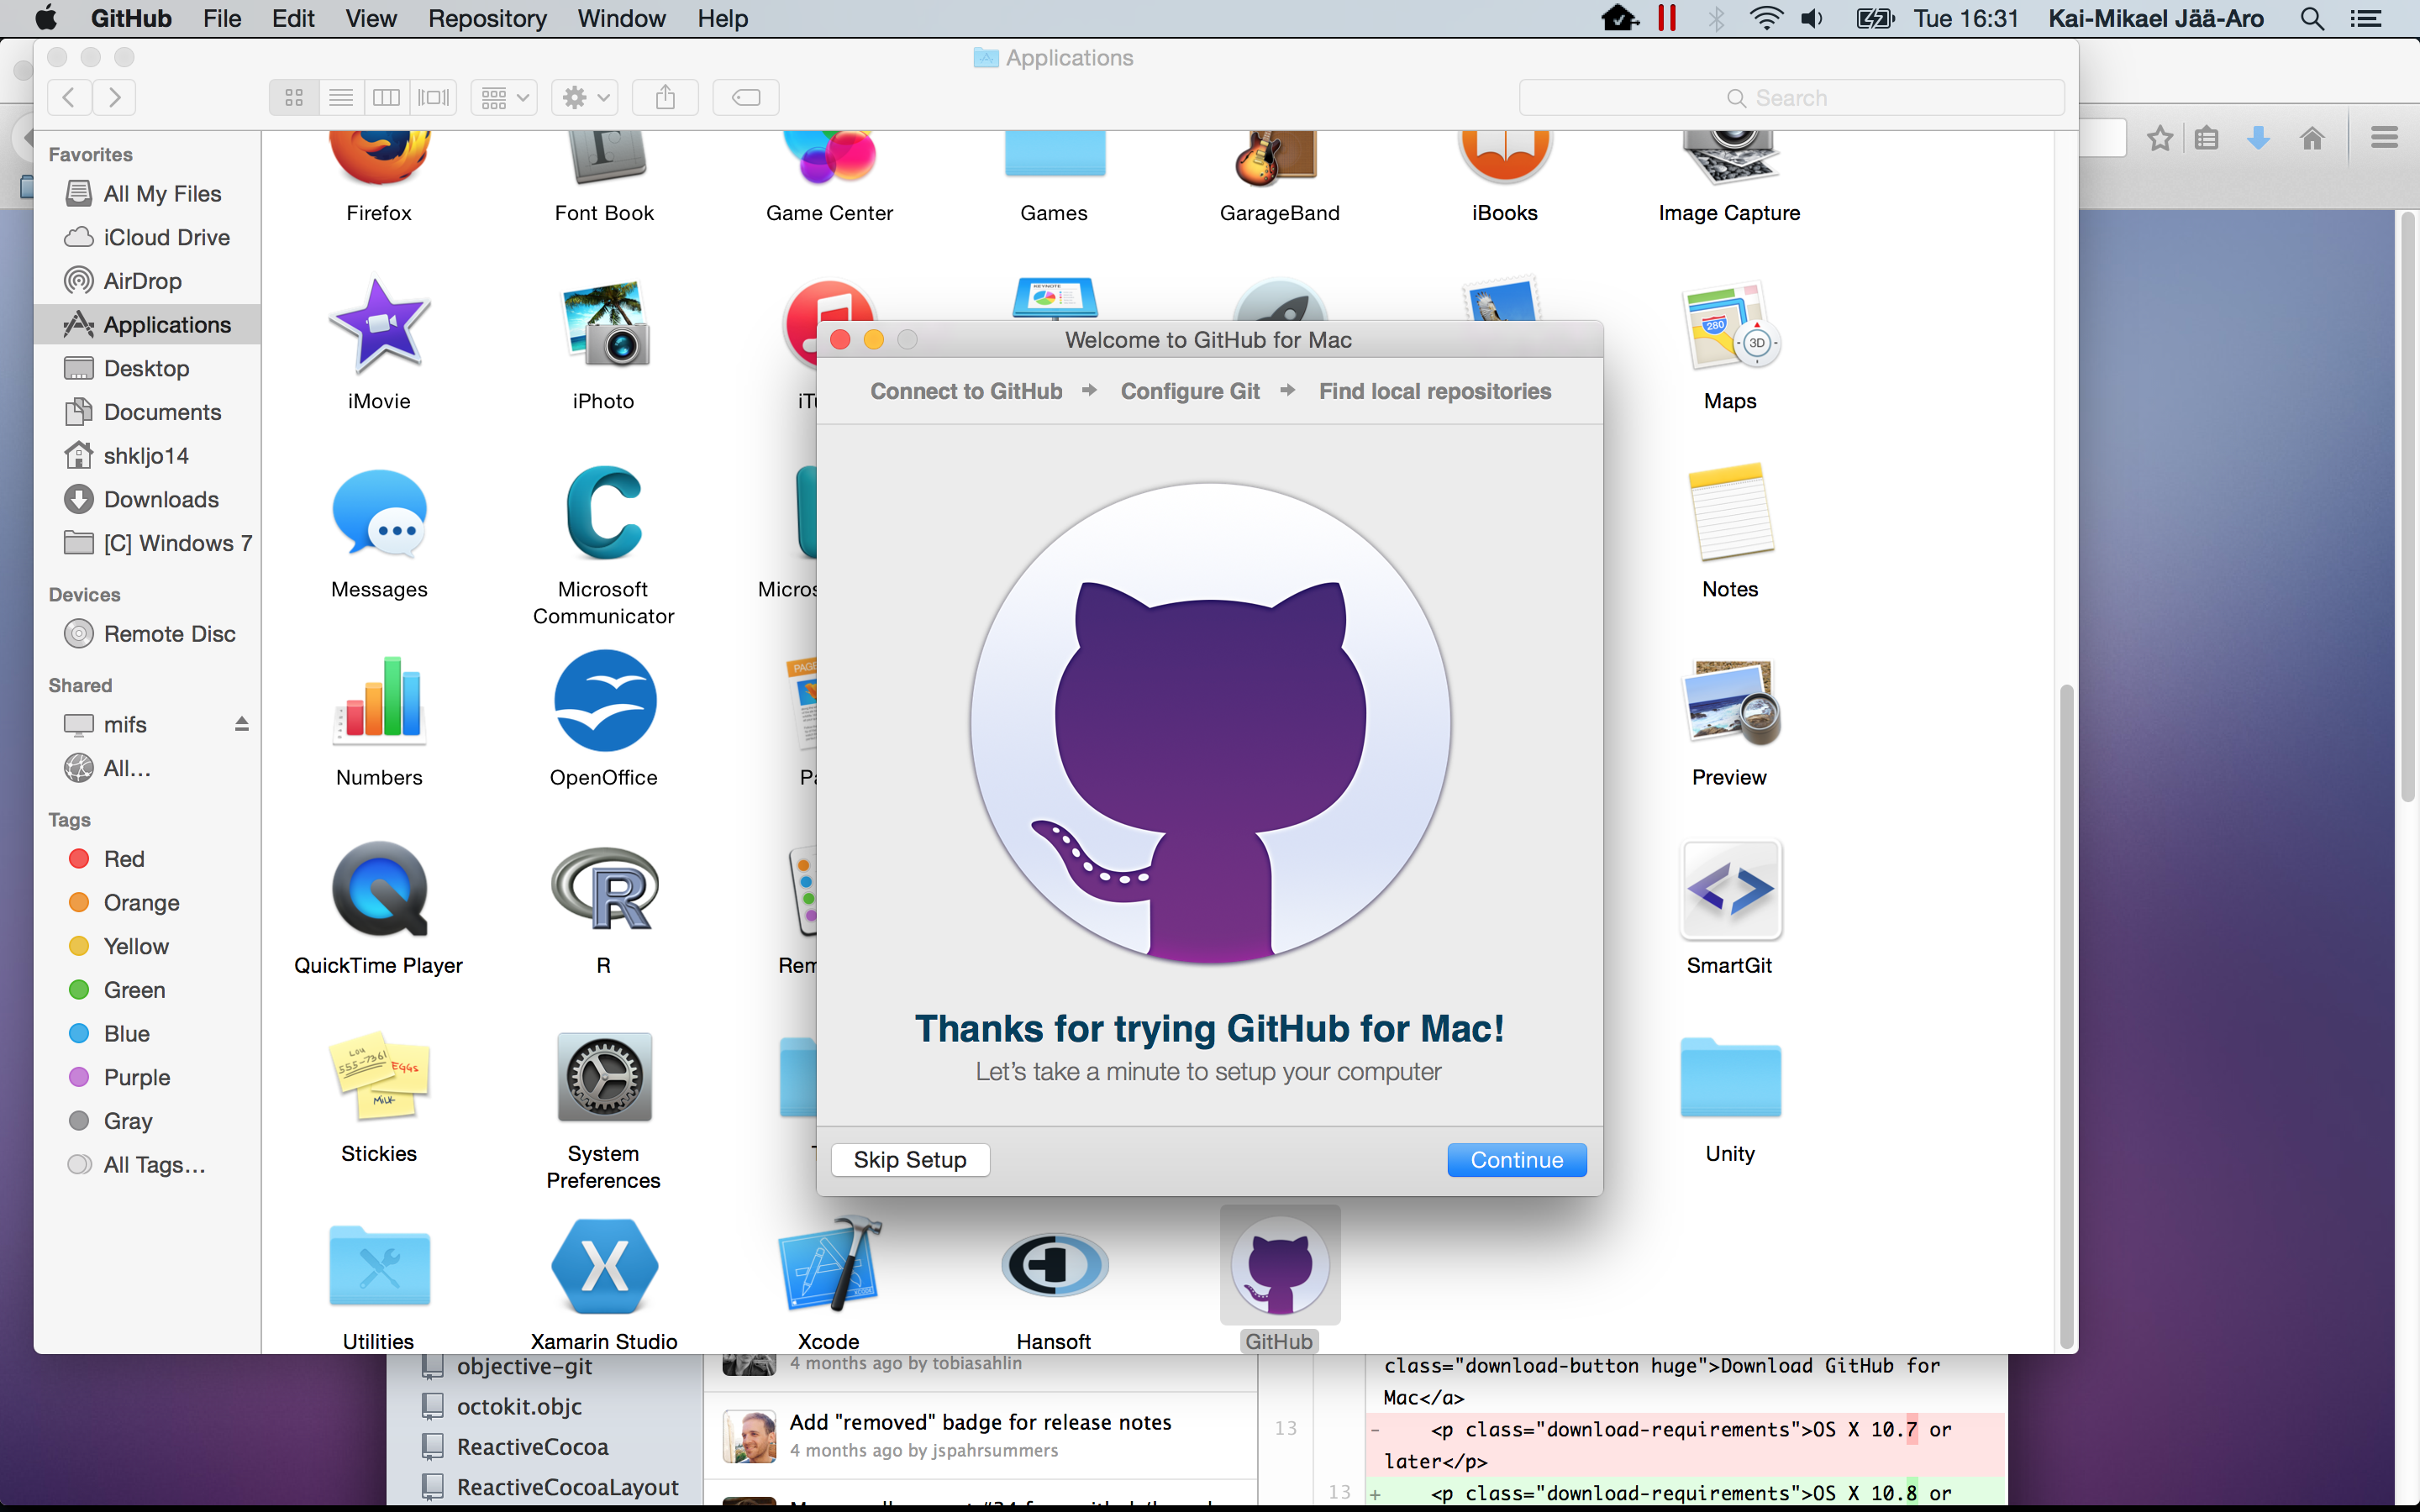
\includegraphics{GitHubWelcome}
\end{frame}

\begin{frame}[fragile]
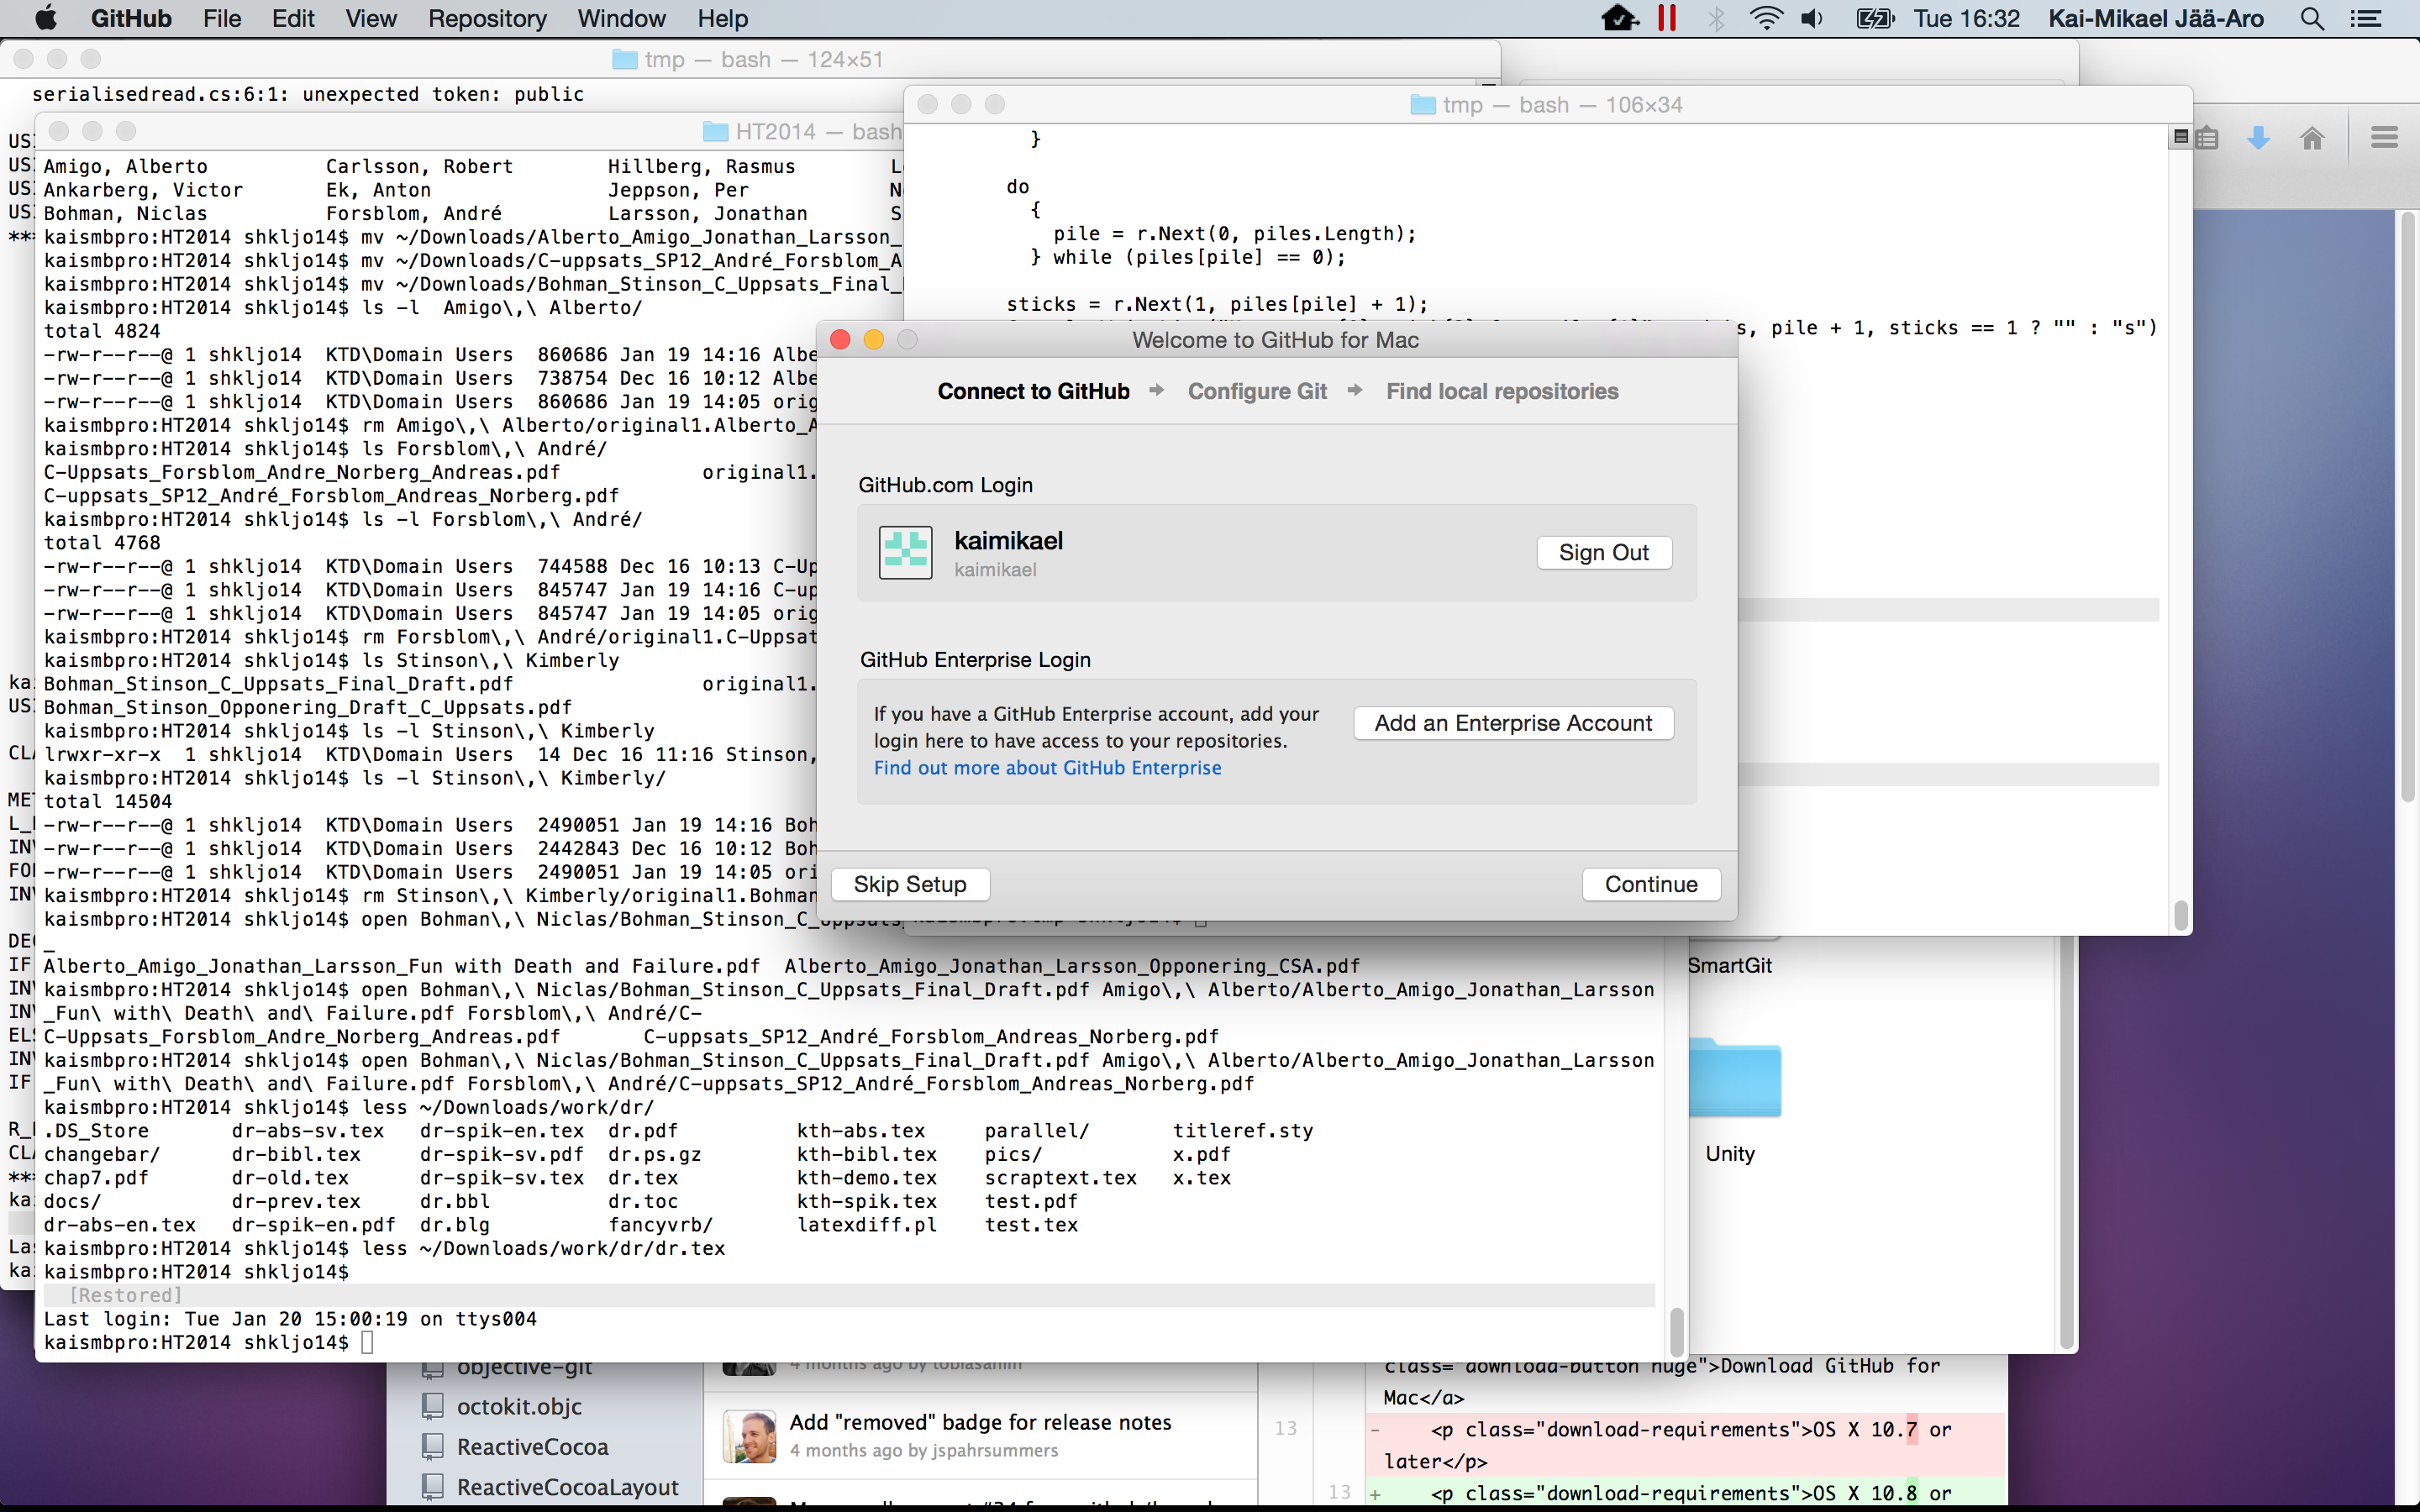
\includegraphics{GitHubLogin}
\end{frame}

\begin{frame}[fragile]
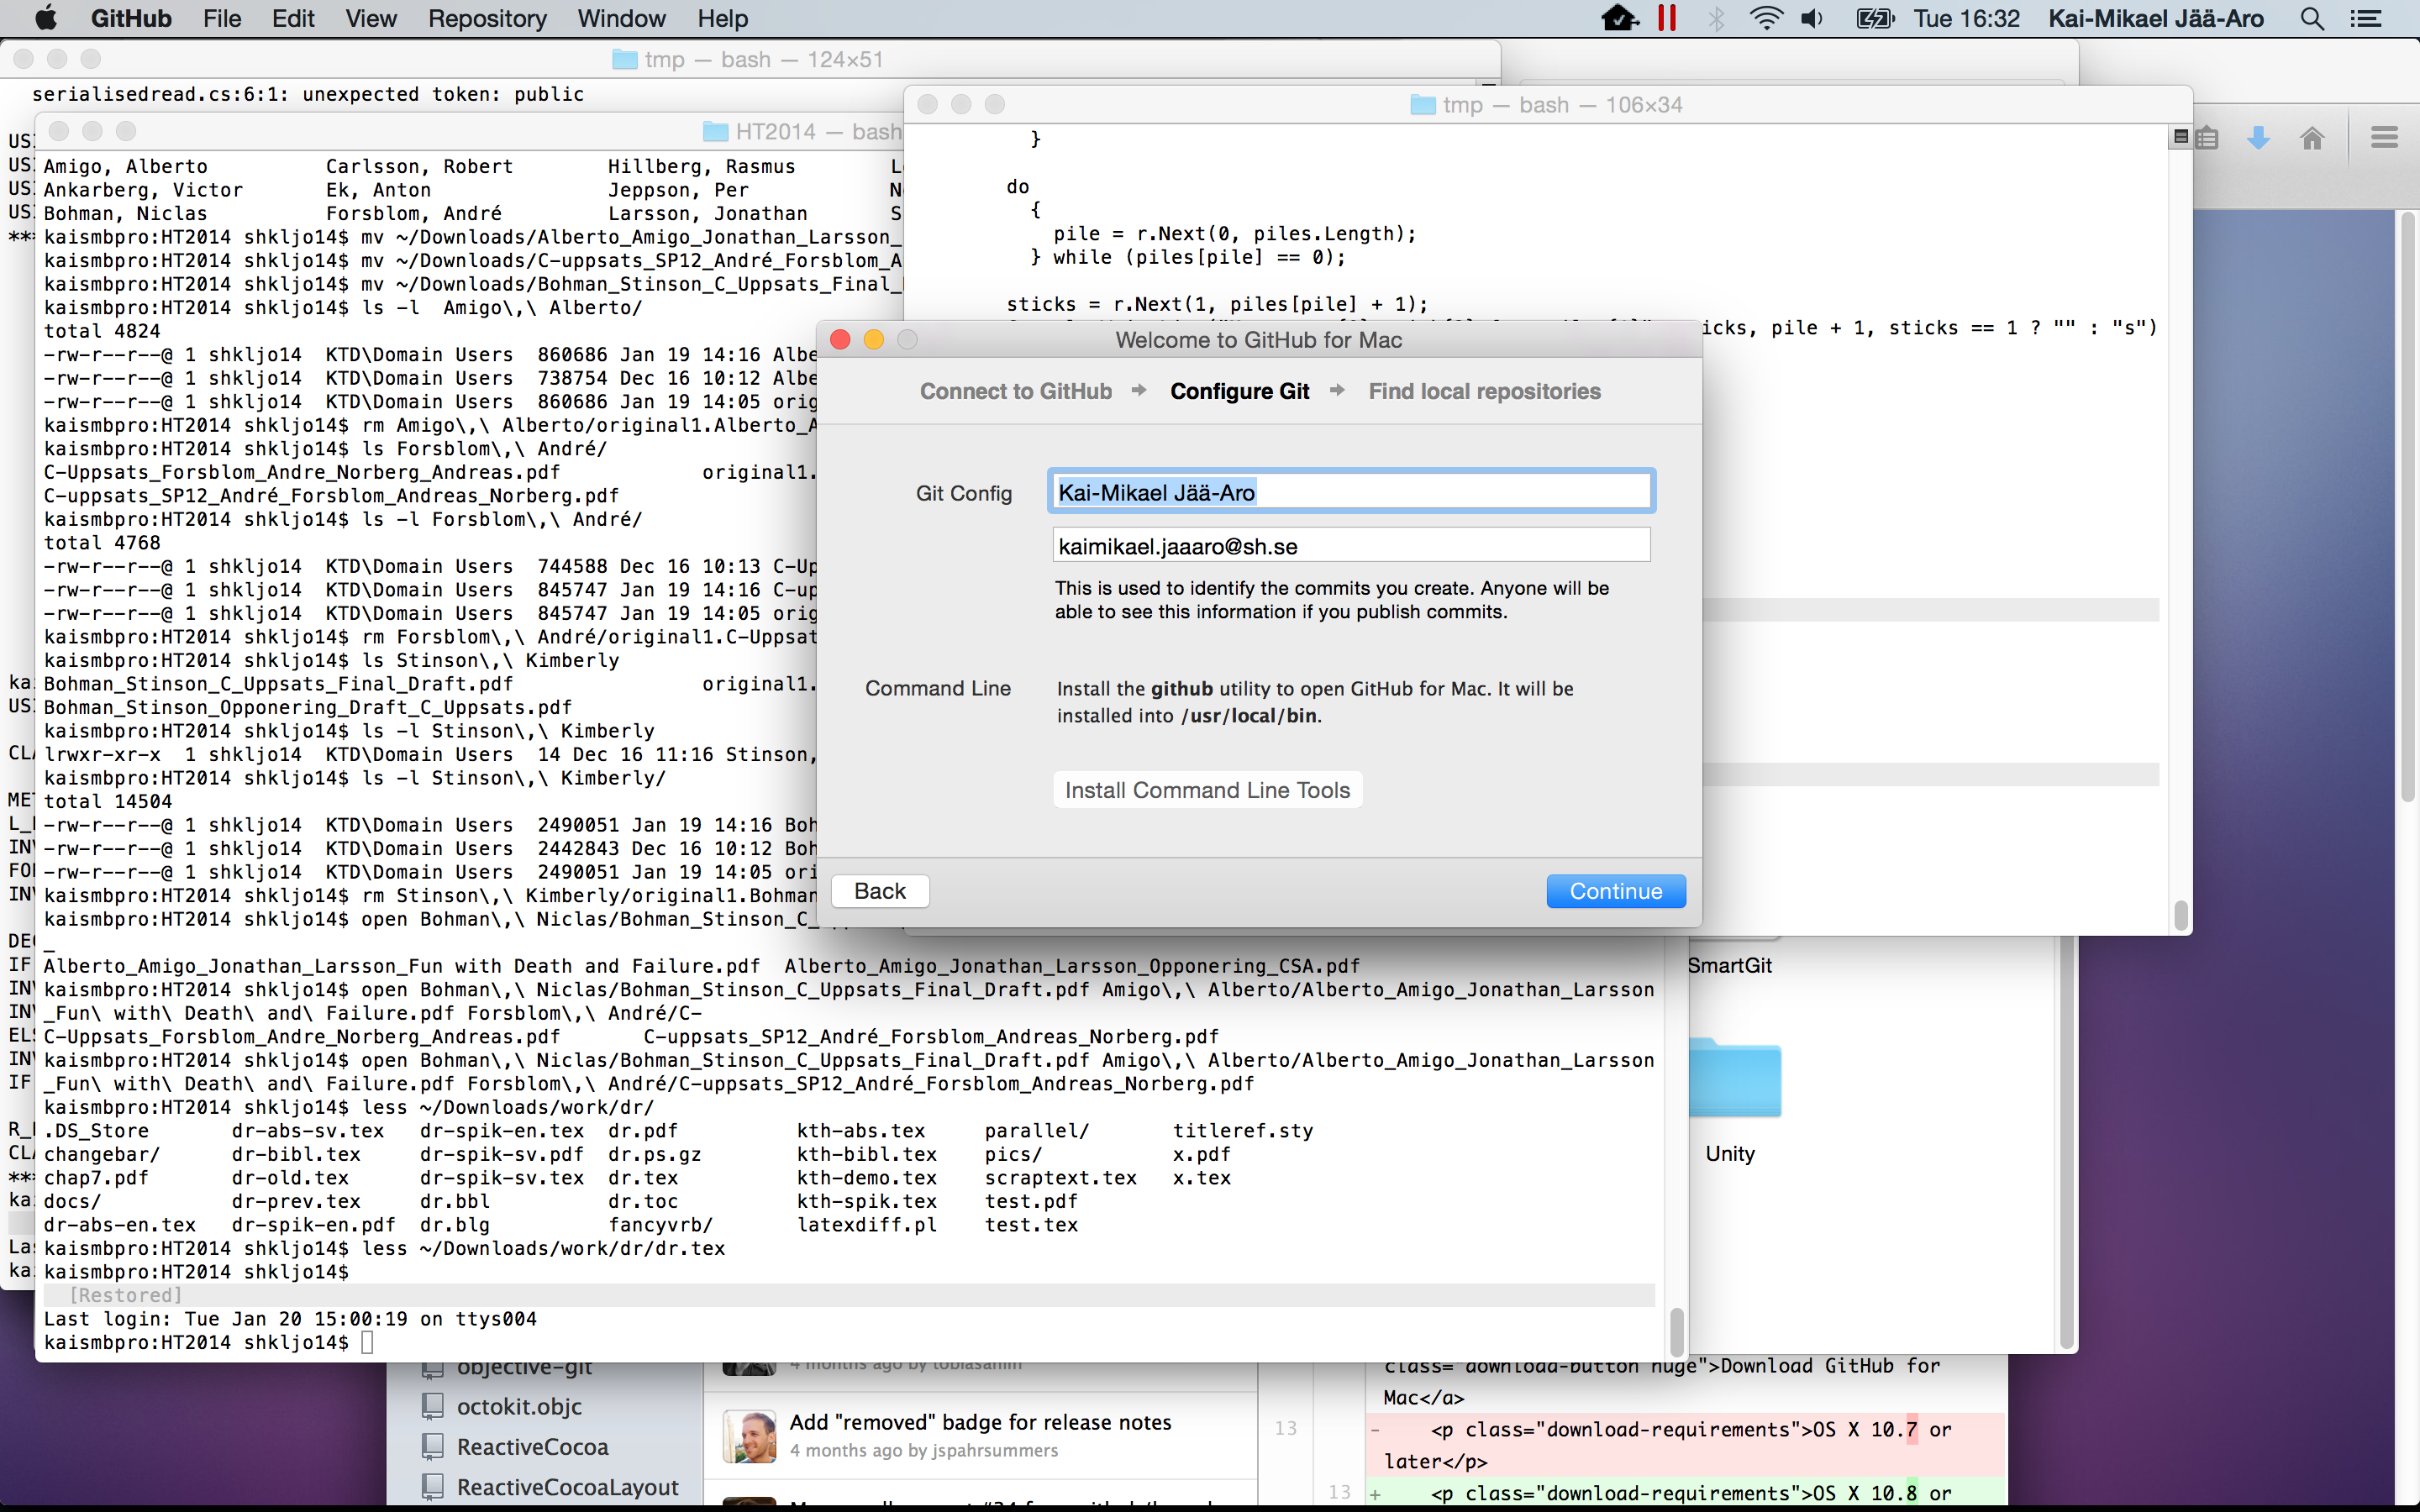
\includegraphics{GitHubConfig}
\end{frame}

\begin{frame}[fragile]
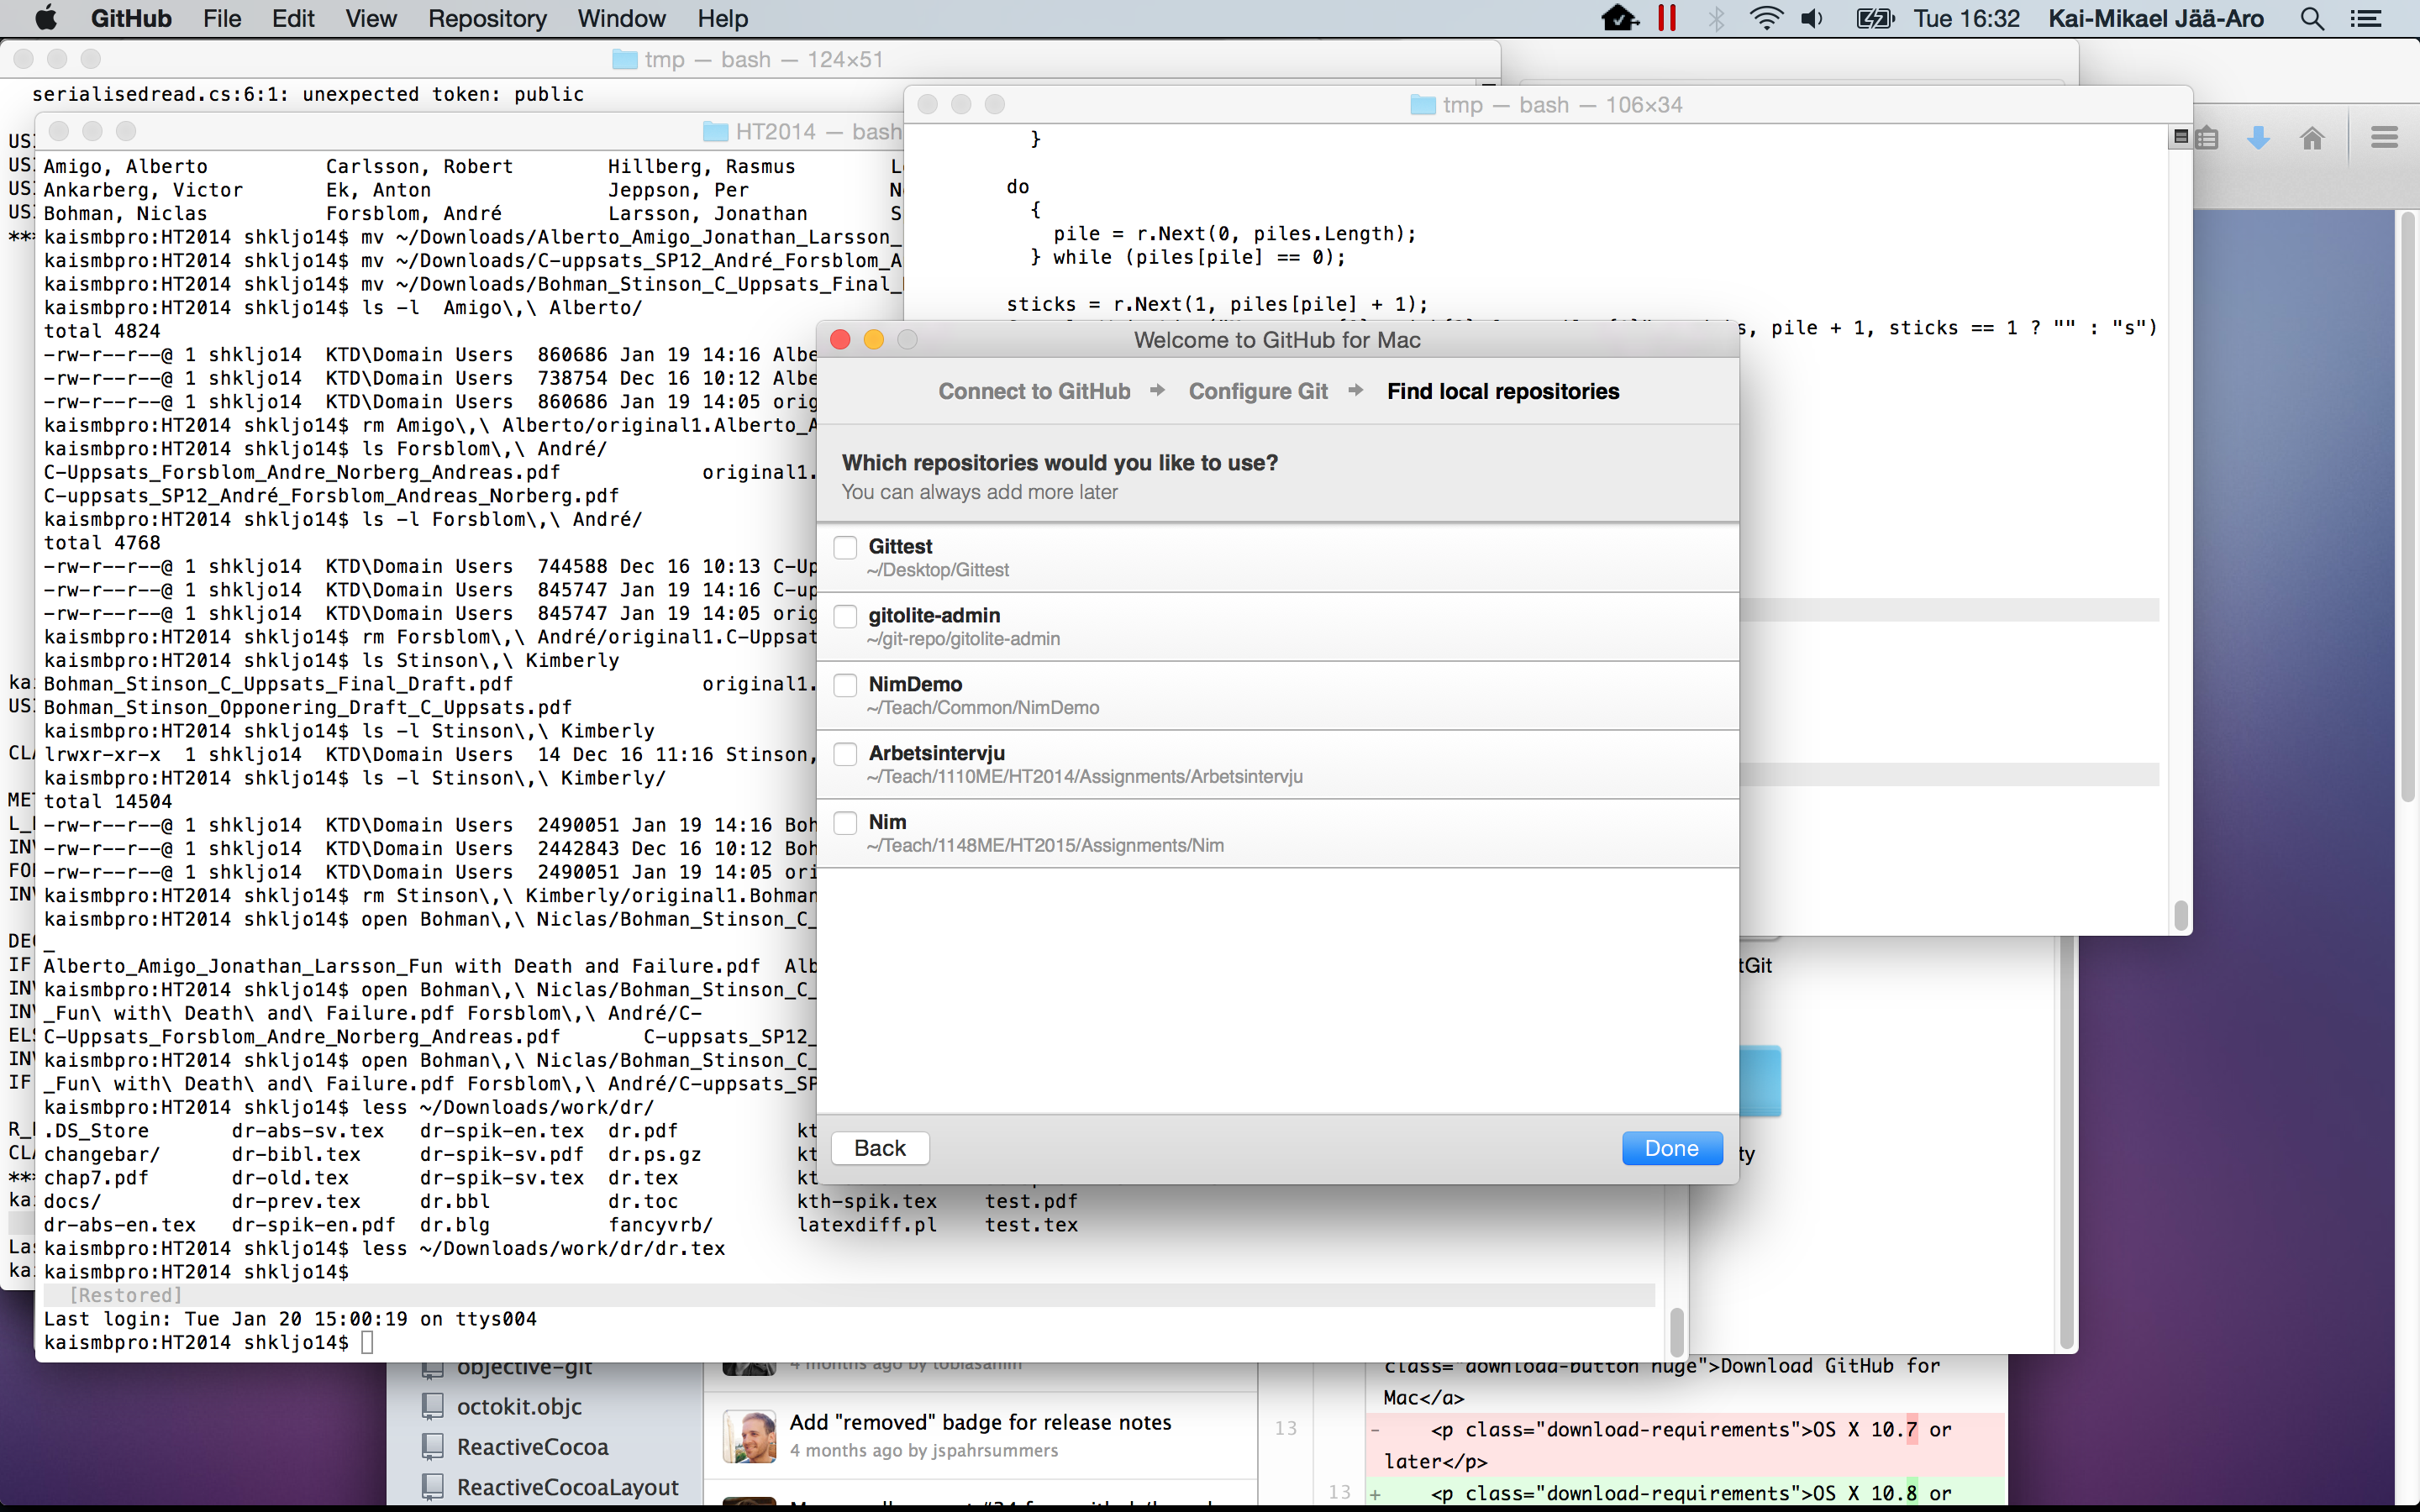
\includegraphics{GitHubFindLocalRepositories}
\end{frame}

\begin{frame}
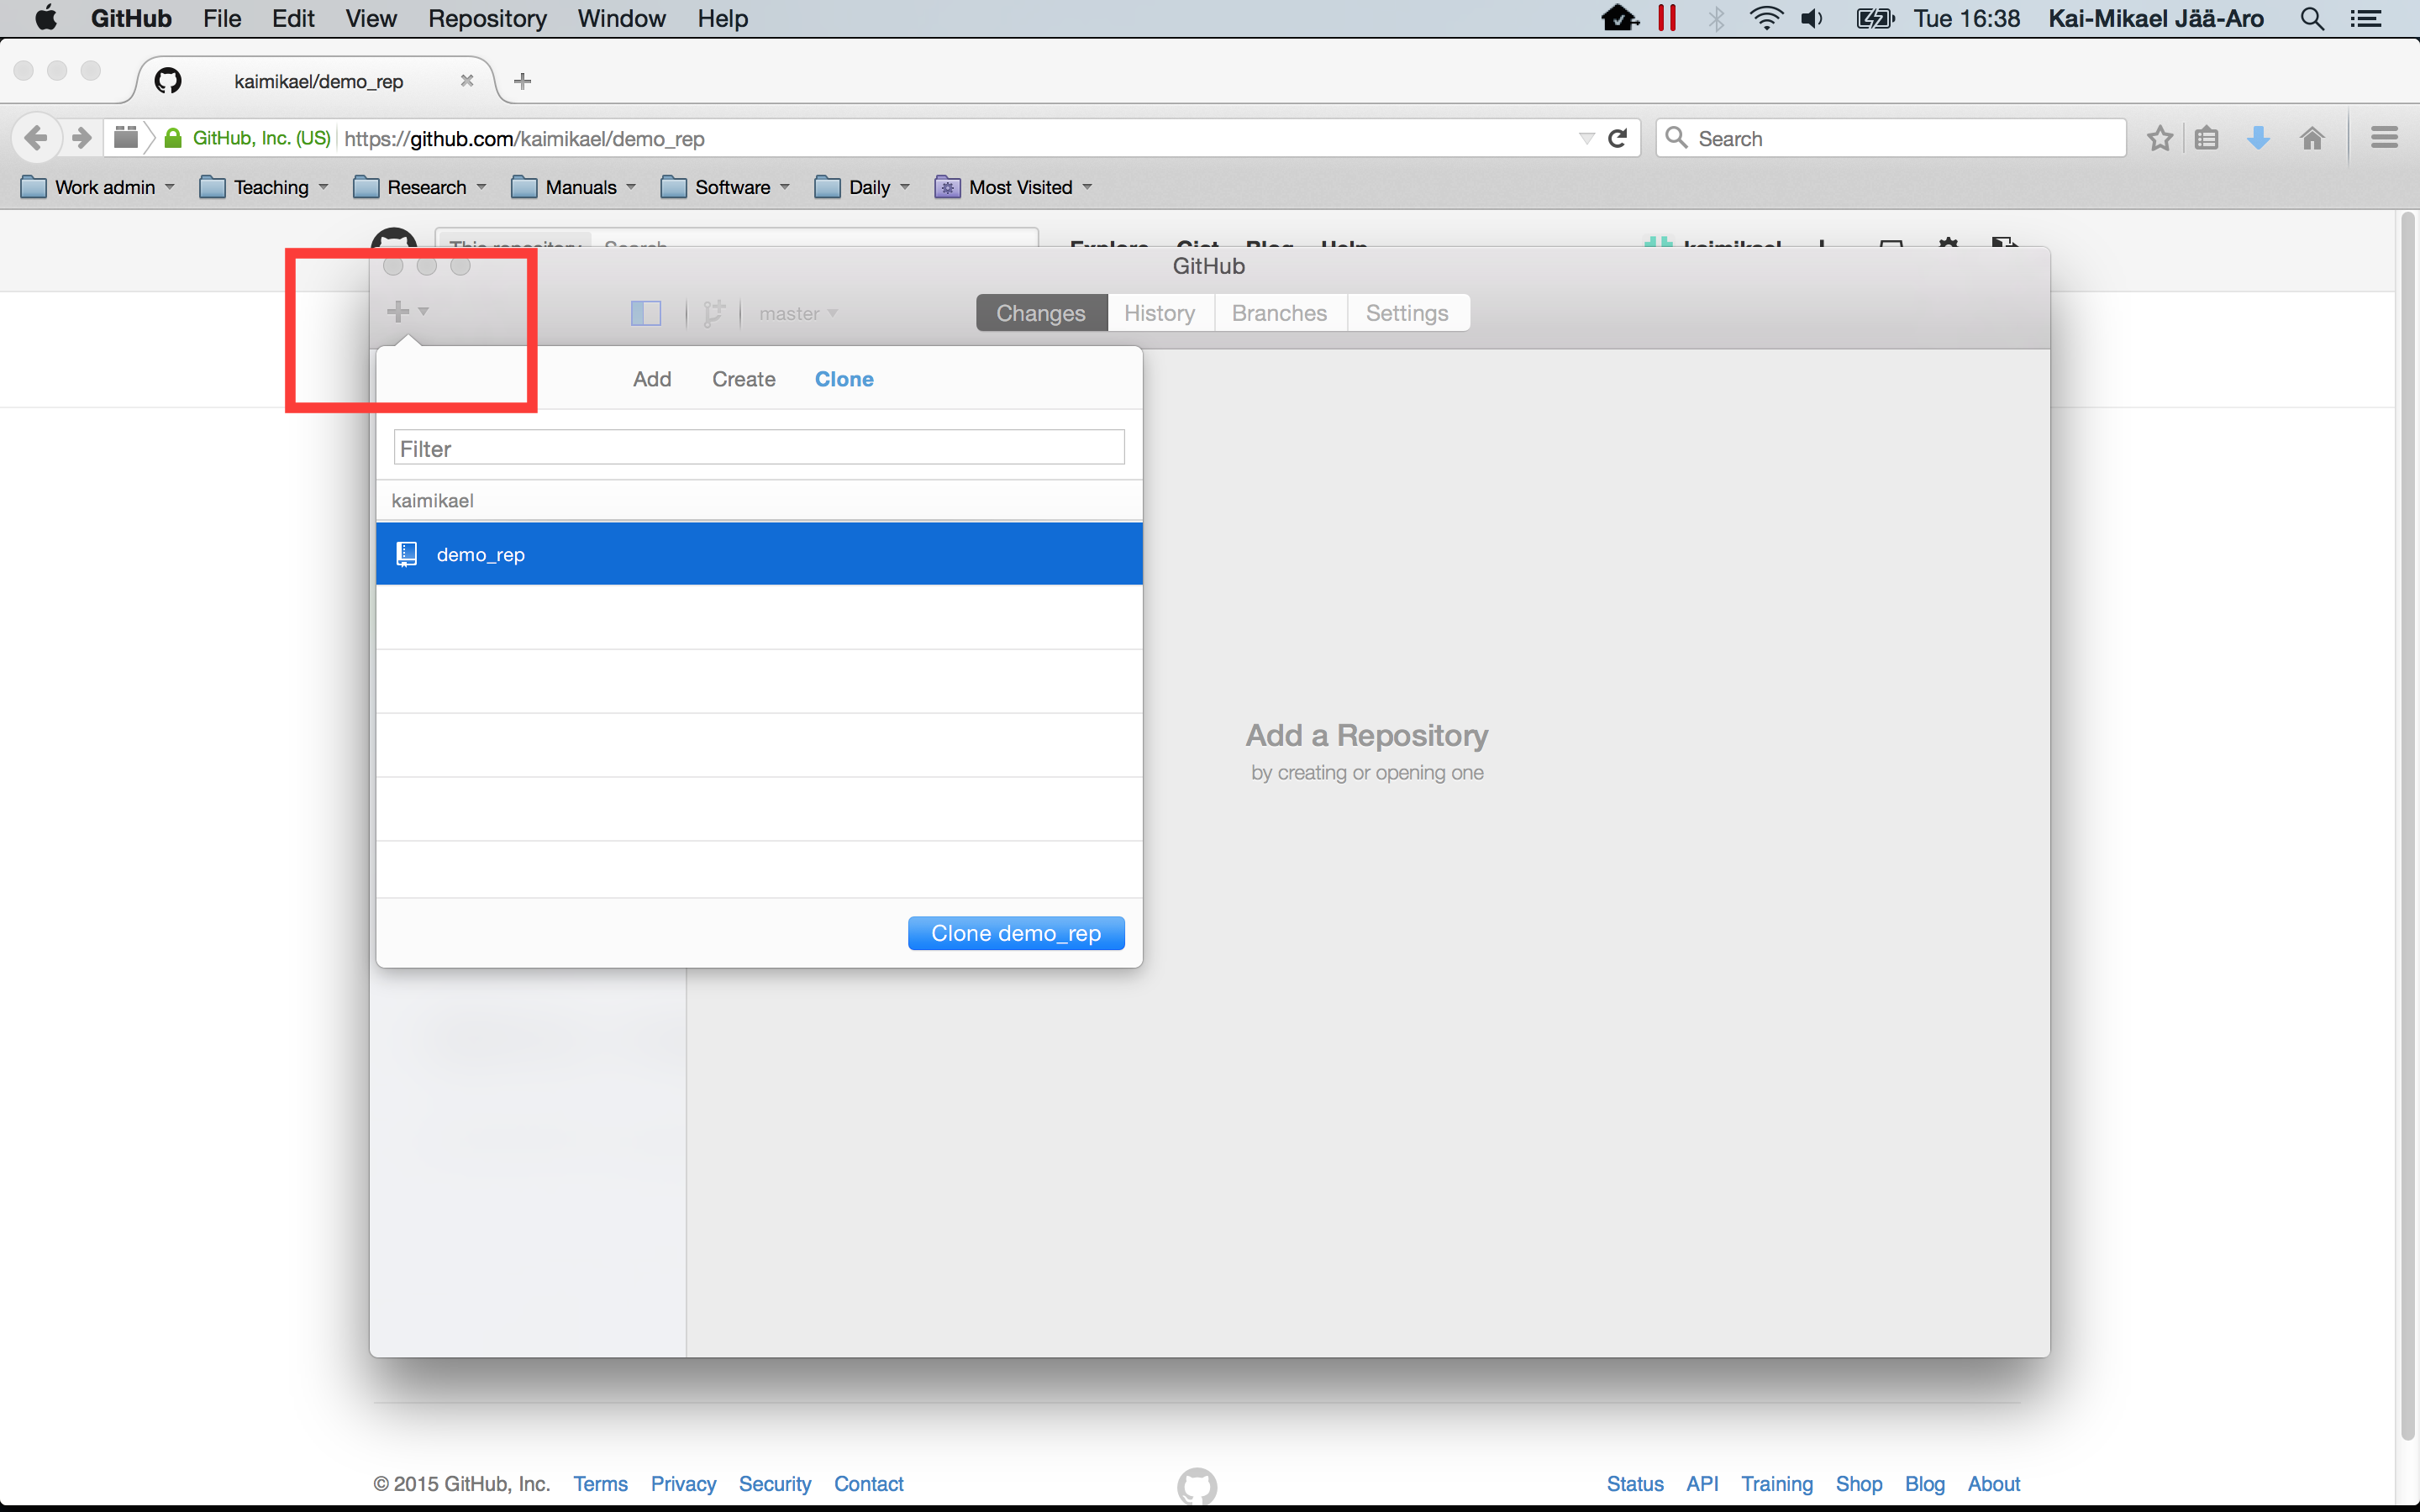
\includegraphics{GitHubCloneRepository}
\end{frame}

\begin{frame}[fragile]
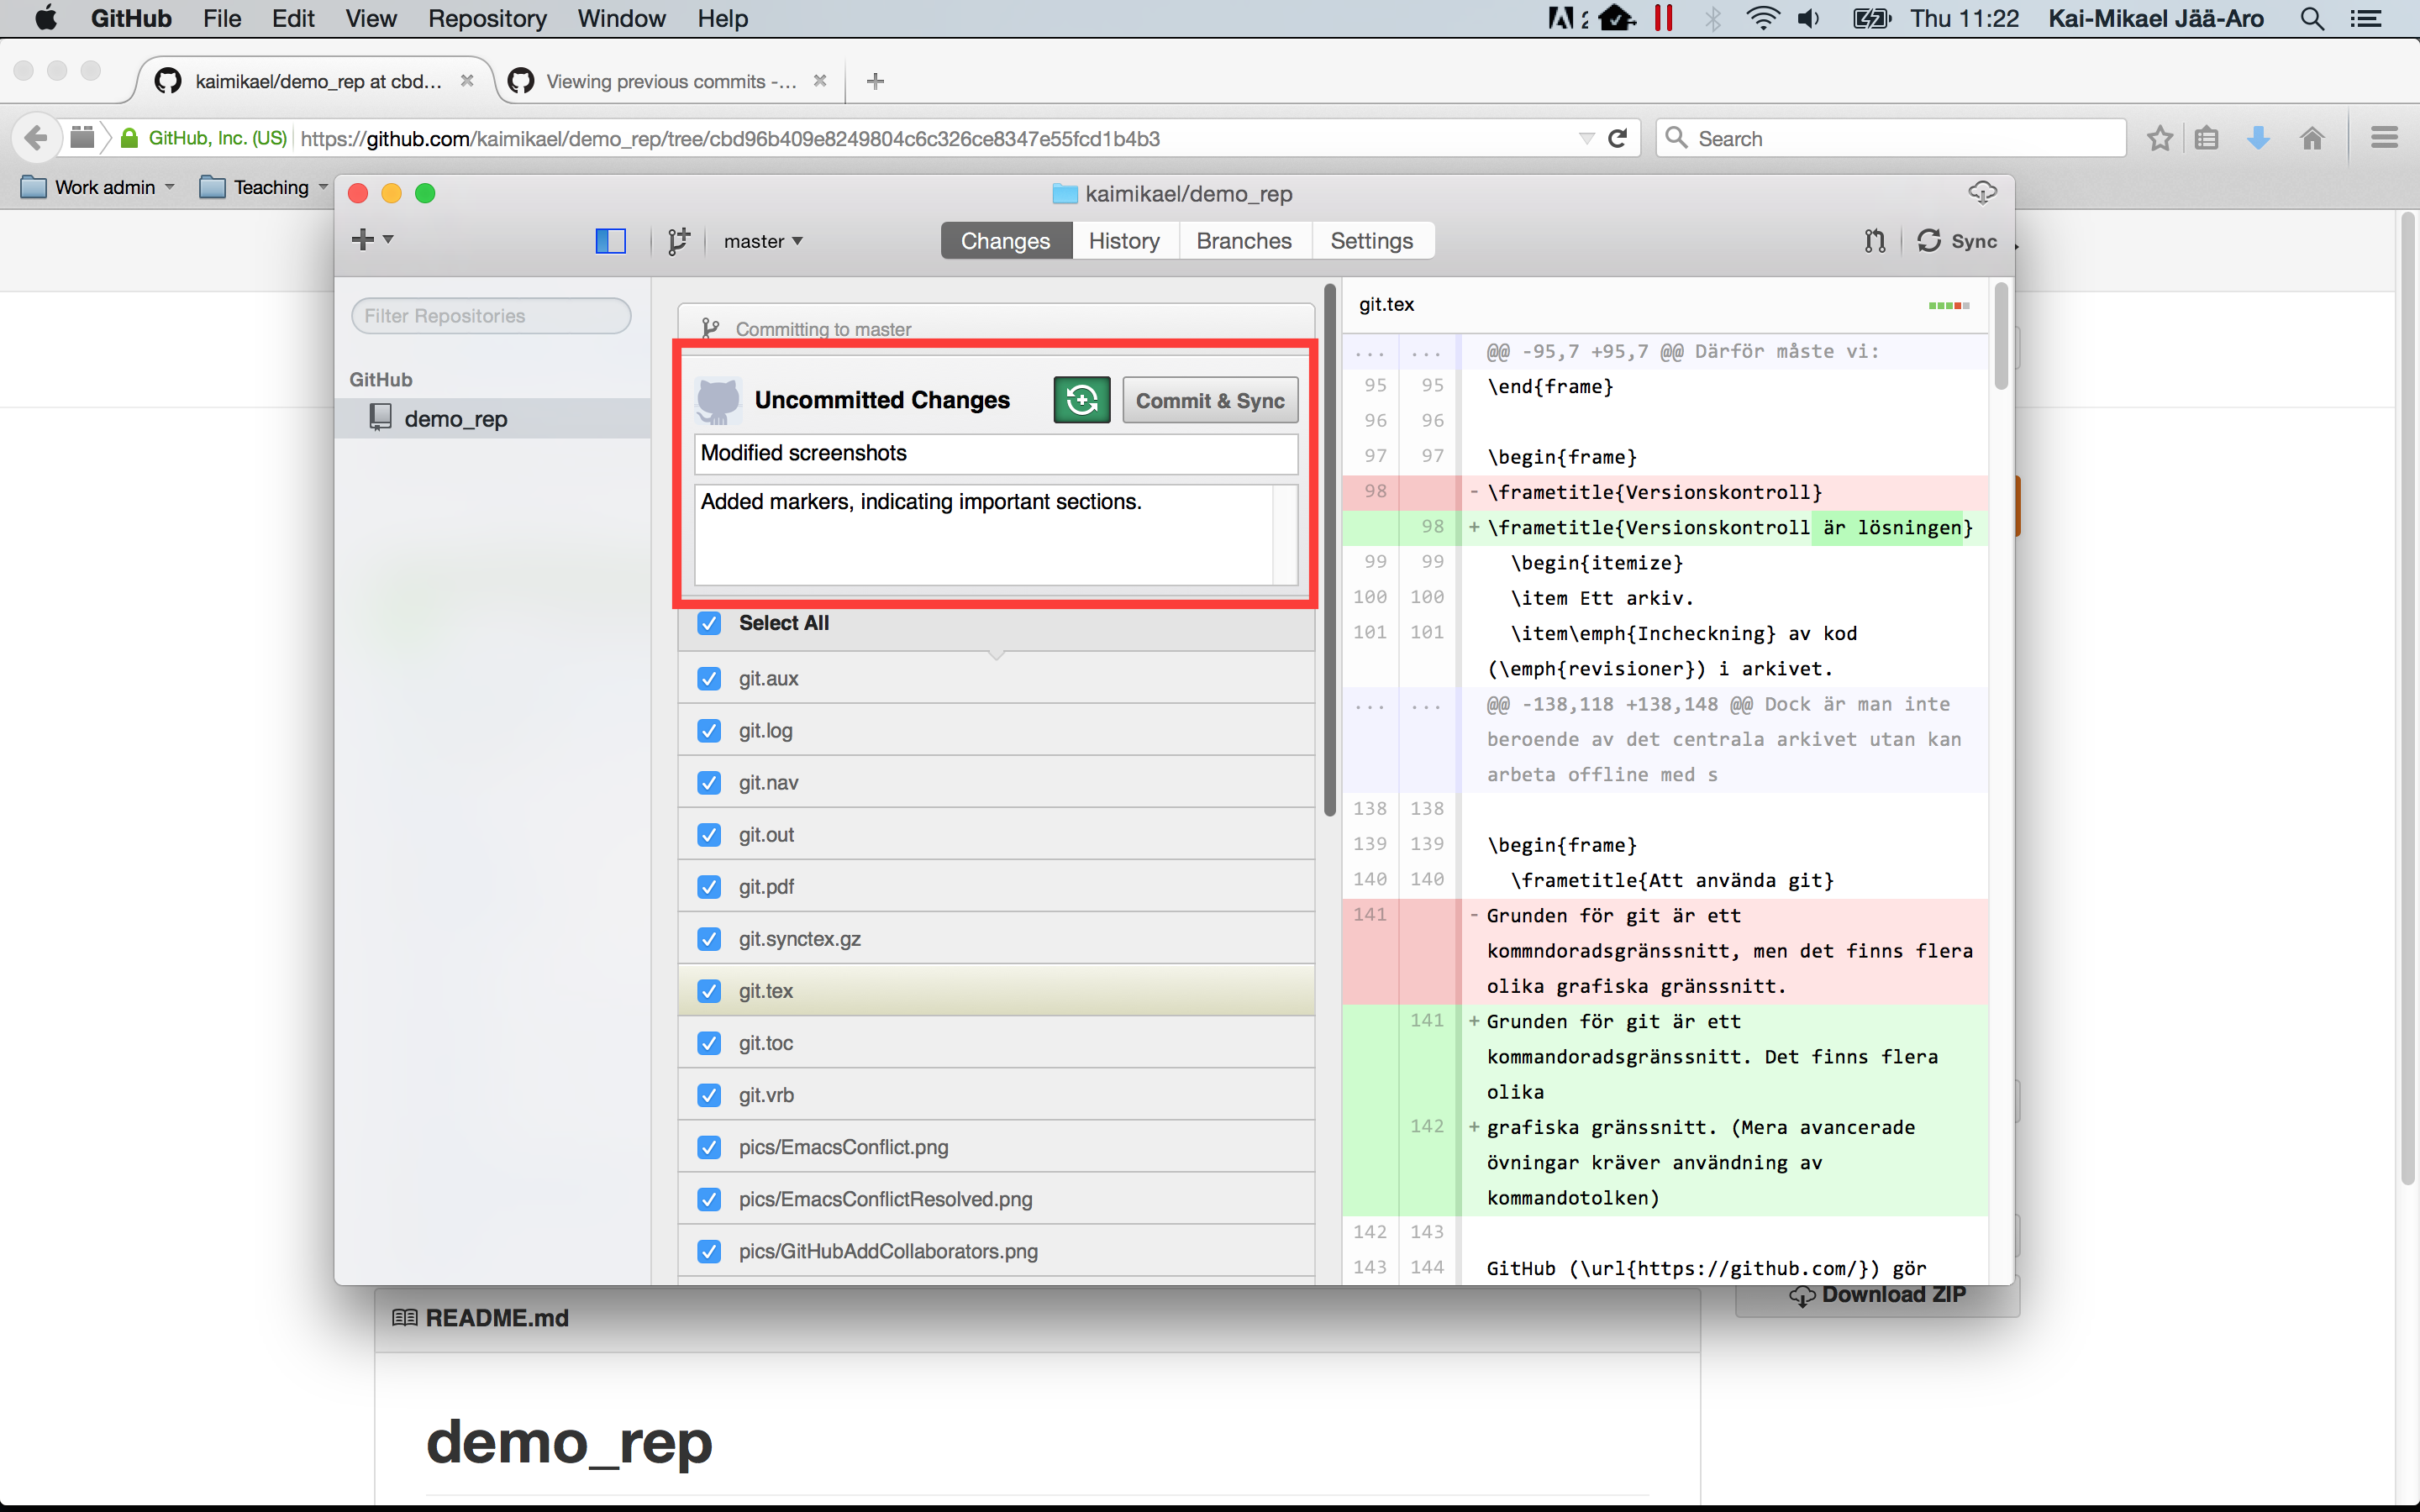
\includegraphics{GitHubAddFiles}
\end{frame}

\begin{frame}[fragile]
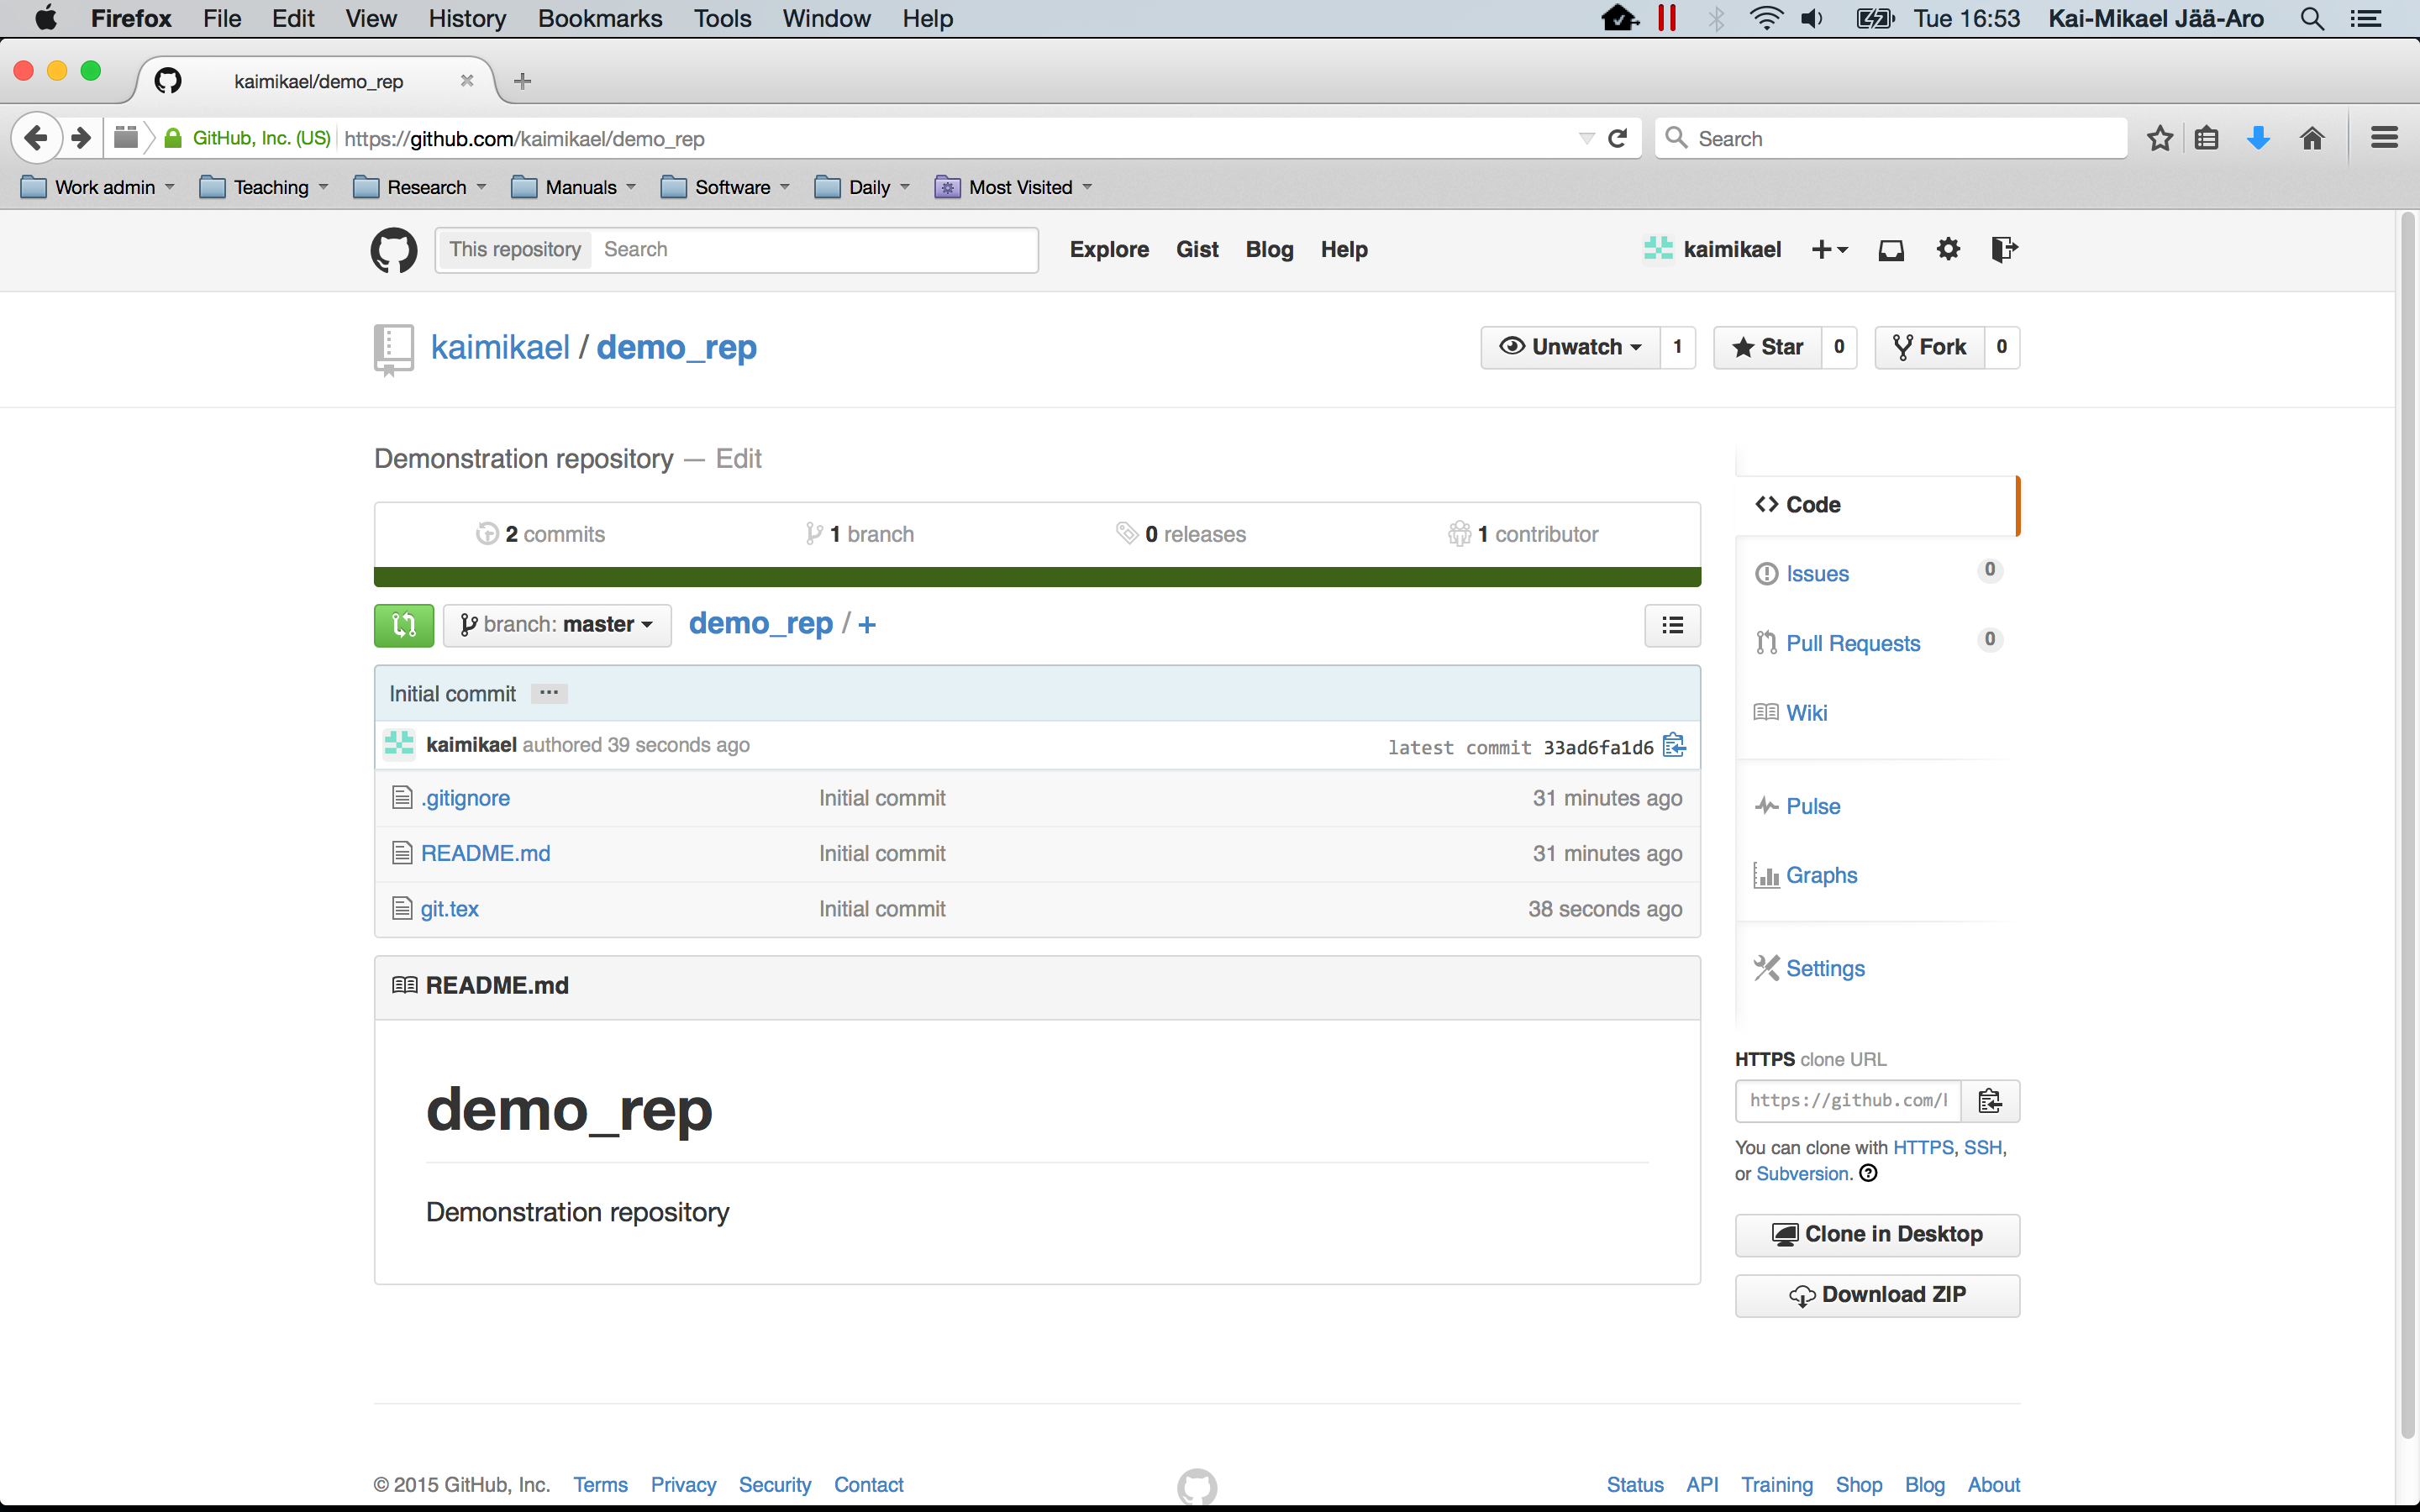
\includegraphics{GitHubWebInterface}
\end{frame}

\begin{frame}[fragile]
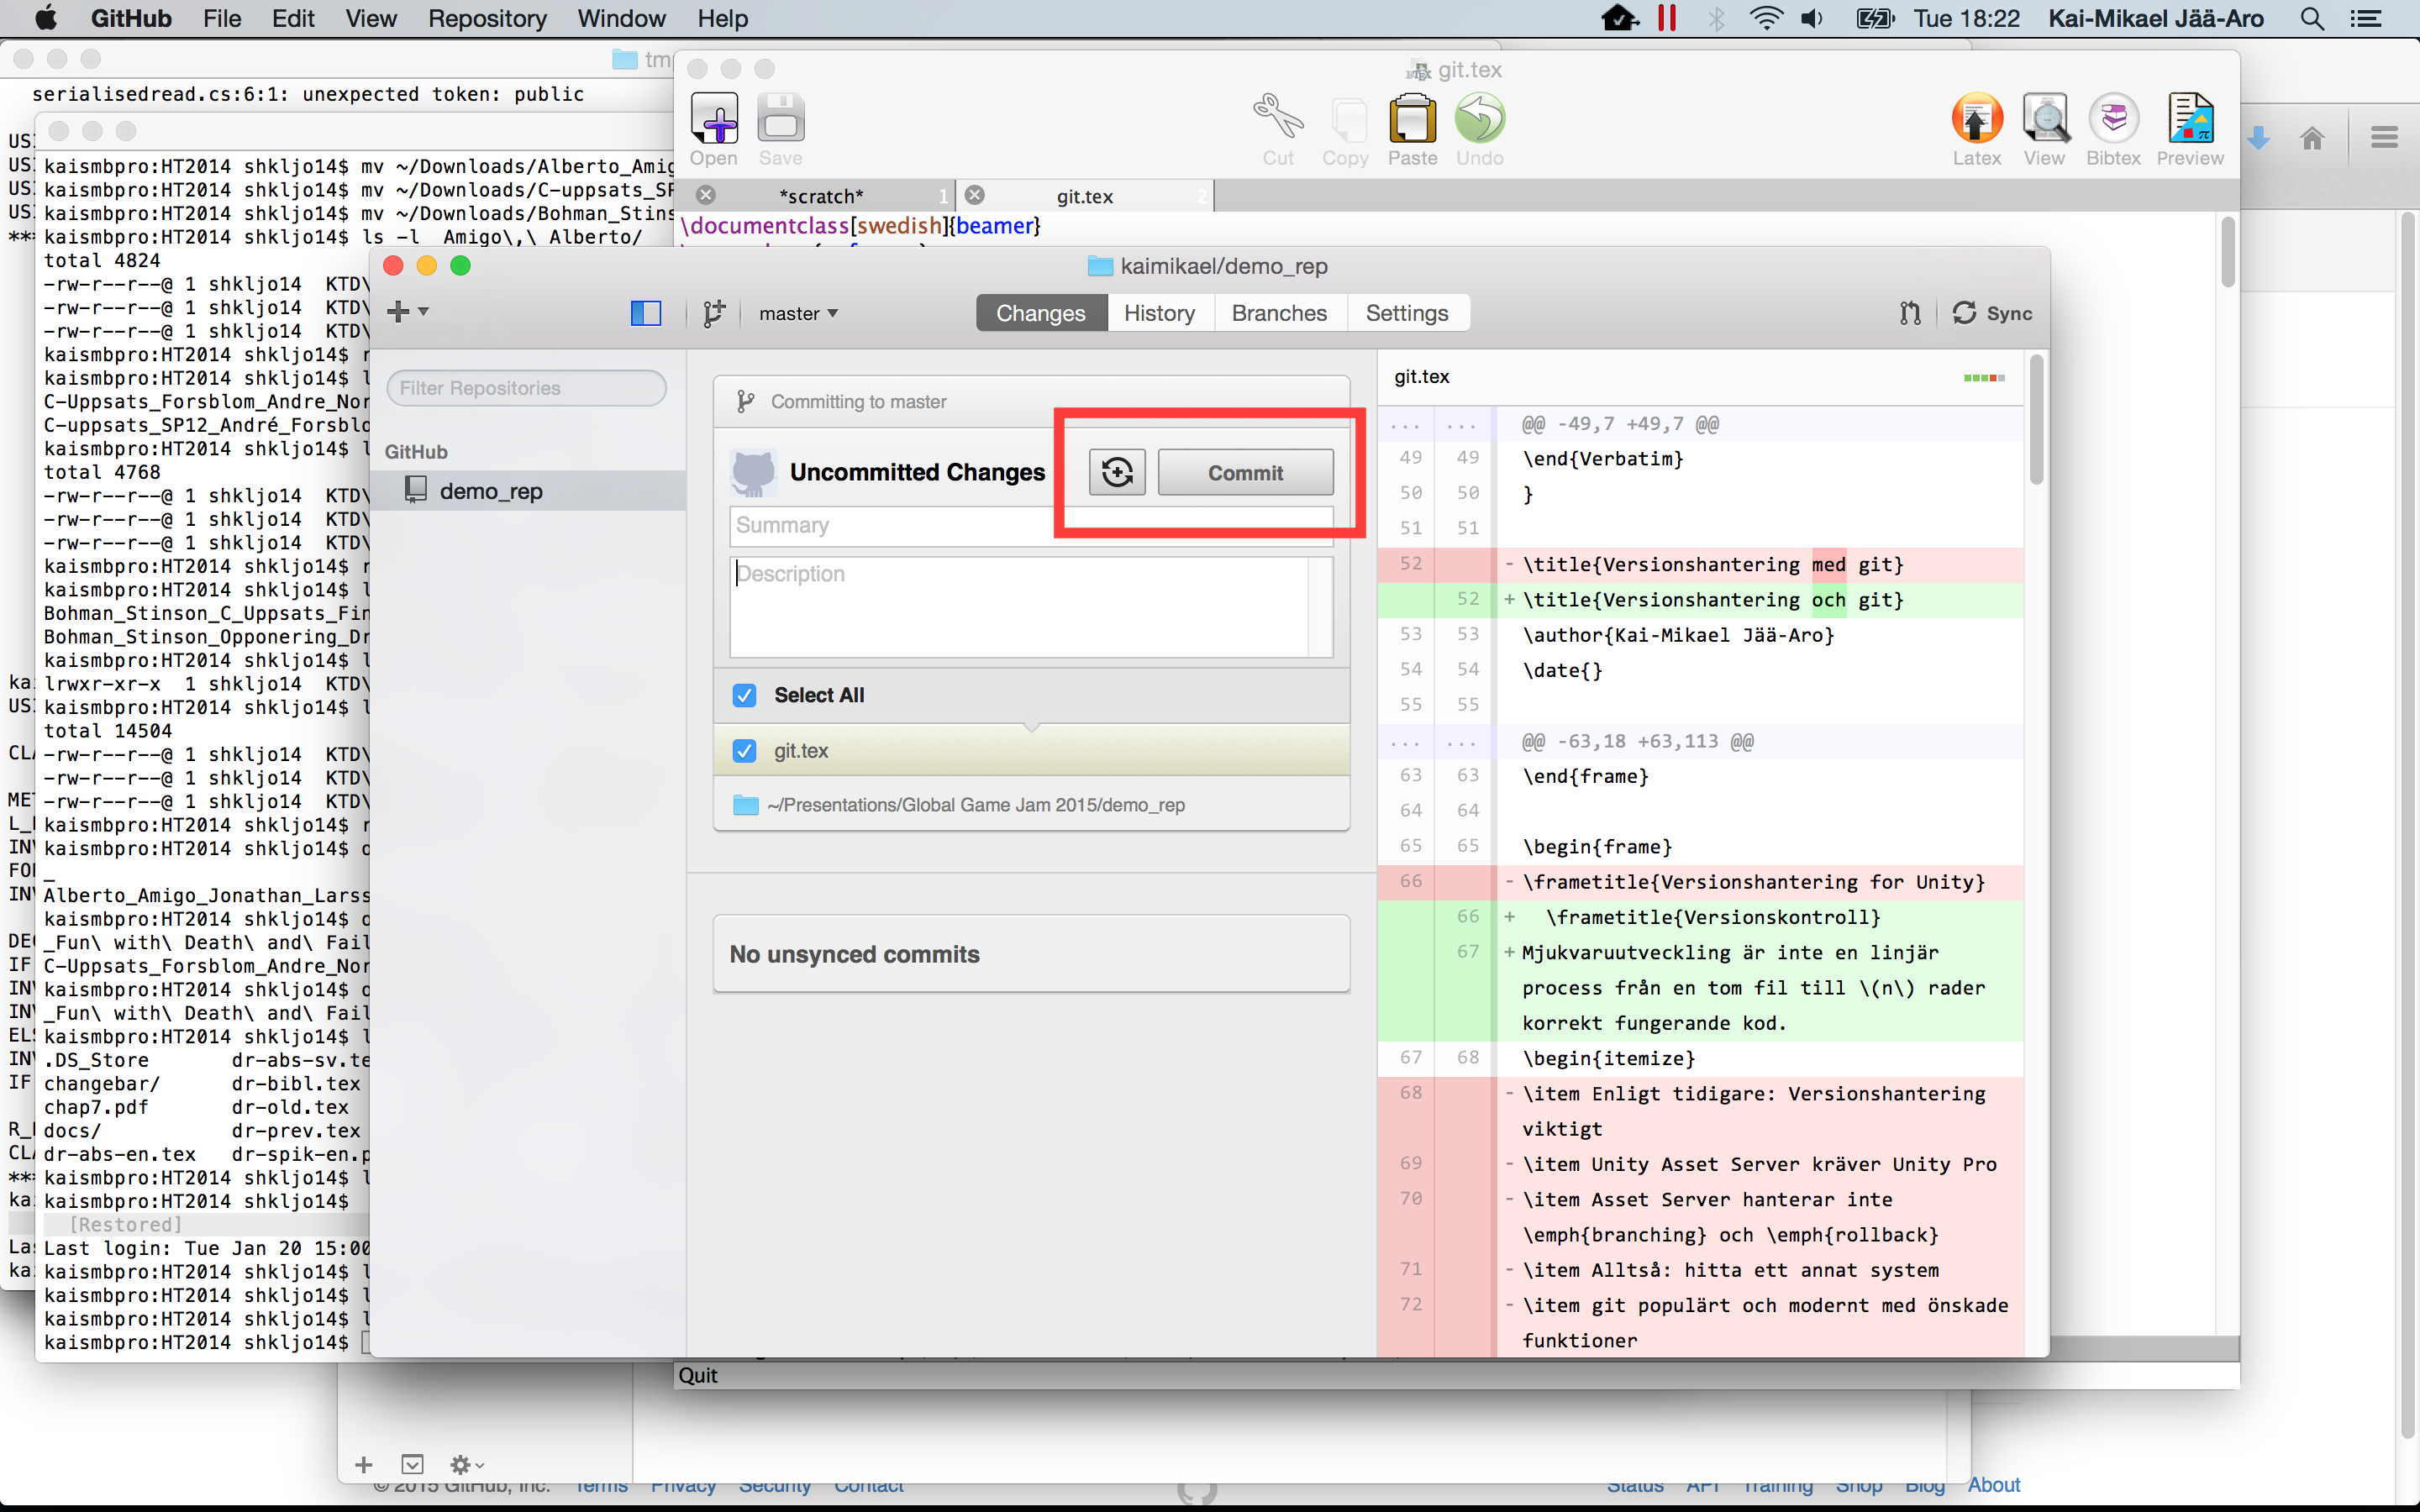
\includegraphics{GitHubCommitChanges}
\end{frame}

\begin{frame}[fragile]
\frametitle{Distribuerad användning}
\end{frame}

\begin{frame}[fragile]

\end{frame}

% \begin{frame}
% \frametitle{Att döpa ett \emph{remote repository}}
% git remote add
% \end{frame}


% \begin{frame}
% \frametitle{Att lagra på ett  \emph{remote repository}}
% git push  
% \end{frame}

% \begin{frame}
% \frametitle{\emph{Tags} och \emph{branches}}
% git tag  
% git push <tagname>

% git branch <branchname>
% git checkout <branchname>
% \end{frame}

\begin{frame}[fragile]
\frametitle{Att ha en privat utvecklingsgren}
Ett vanligt arbetsflöde är att man har en \emph{master branch}, där koden är garanterad att vara stabil och körbar.  Olika utvecklare kan sedan lätt skapa en egen gren att koda och testa i.  Om något blir fel kan man alltid backa i denna gren och hålla mastern stabil.  Man kan självfallet göra ytterligare grenar för olika tester.

git-arkiven är uppbyggda så att de låter oss arbeta på vilken punkt i trädet vi vill.  Man kan se det som att man har en pekare in i trädet som pekar ut den aktuella uppsättningen filer som vi arbetar på.  Vid behov kan vi flytta pekaren nån annanstans och arbeta där istället.
\end{frame}

\begin{frame}[fragile]
  \begin{columns}
    \begin{column}{0.5\textwidth}
      Vi skapar en branch med 
      \begin{dialogue}
prompt> #textbf(git branch #textit(branchnamn))
      \end{dialogue}
och säger att vi vill arbeta med en specific branch
\begin{dialogue}
prompt> #textbf(git checkout #textit(branchnamn))  
\end{dialogue}
Vi hamnar då i ''spetsen'' av den aktuella grenen.
    \end{column}
    \begin{column}{0.5\textwidth}
\menu{Add Branch}

\vspace{\baselineskip}

\includegraphics[width=\textwidth]{BranchAndCheckout}
    \end{column}
  \end{columns}
  
\end{frame}

\begin{frame}[fragile]
\frametitle{\emph{Merge}}
\begin{columns}
\begin{column}{0.5\textwidth}
När man har en utvecklingsversion man är nöjd med är det dags att koppla ihop den med mastern.  
\begin{dialogue}
prompt> #textbf(git checkout master)
prompt> #textbf(git merge otherbranch)
\end{dialogue}

git kommer nu att försöka kombinera filerna från bägge grenarna.
\end{column}
\begin{column}{0.5\textwidth}
\menu{Merge}

\vspace{\baselineskip}

\includegraphics[width=\textwidth]{Merge}

\end{column}
\end{columns}
\end{frame}

\begin{frame}[fragile]
    Det kan vara så att det finns konflikter (överlappande ändringar) i koden, så att man måste gå igenom manuellt och välja vilket av de möjliga alternativen som ska användas.  Då kan man ta hjälp av 
\begin{dialogue}
prompt> #textbf(git mergetool)
\end{dialogue}
(kan kräva installation av lämplig mjukvara).

Om man inser att man gjort bort sig fullständigt, kan man ångra sig:
\begin{dialogue}
prompt> #textbf(git merge --abort)
\end{dialogue}

Till sist, när allt är OK, så gör man en commit.
\end{frame}
\begin{frame}[fragile]
\frametitle{\emph{merge} av binära filer}
git klarar inte (idag) av att göra merge på binära filer -- \mao texturer, animationer, \odyl.  Somliga installationer kan ha en mergetool som kan hjälpa till, men i allmänhet måste man manuellt hämta de binära filer man vill ha med 
\begin{dialogue}
prompt> #textbf(git checkout #textit(treeish) #textit(filnamn))  
\end{dialogue}
  
\end{frame}


\begin{frame}[fragile]
\frametitle{Mer läsning}  
\href{http://git-scm.com/book/en/v2/}{\textsl{Pro Git, 2nd Edition}, Scott Chacon \& Ben Straub.}
\begin{dialogue}
prompt> #textbf(man git)
\end{dialogue}
\end{frame}
\end{document}
